
A separate maximum-likelihood fit is performed over the 1-jet and 2-jet fit regions in order to extract the best-fit value of the WZ + b-jet and WZ + charm jet contributions. The $WZ$ + b, $WZ$ + charm and $WZ$ + light contributions are allowed to float, with the remaining background contributions are held fixed. \textbf{The current fit strategy treats the WZ + b-jet contribution as the parameter of interest, with the normalization of the $WZ$ + charm and the $WZ$ + light contributions taken as systematic uncertainties. This could however be adjusted, depending on whether it is decided the goal of the analysis should be to measure WZ+b specifically or WZ + heavy flavor overall.} The result of the fit is used to extract the cross-section of $WZ$ + heavy-flavor production.

A maximum likelihood fit to data is performed simultaneously in the regions described in section \ref{sec:evt_selection}. The parameters $\mu_{WZ+b}$, $\mu_{WZ+charm}$, $\mu_{WZ+light}$, where $\mu = \sigma_{observed}/\sigma_{SM} $, are extracted from the fit.

%While in the nominal fit events with an intermediate top quark are treated as a separate process, an alternative version of the measurement is performed which considers tZ as part of the signal.

The Asimov fit for 1-jet events gives an expected $\mu$ value of $1.00^{+0.37}_{-0.35}(stat)^{+0.24}_{-0.22}(sys)$ for $WZ$ + b. The fitted cross-section modifiers for $WZ$ + charm and $WZ$ + light are $1.00 \pm 0.17 \pm 0.15$ and $1.00 \pm 0.04 \pm 0.07 $, respectively.

The expected cross-section of WZ+b with 1 associated jet obtained from the fit is $1.74^{+0.65}_{-0.61}(stat)^{+0.42}_{-0.37}(sys)$ fb with an expected significance of 2.2$\sigma$.

For 2-jet events, the fit gives an expected $\mu$ value of $1.00^{+0.34}_{-0.33}(stat)^{+0.29}_{-0.28}(sys)$ for $WZ$ + b. The fitted cross-section modifiers for $WZ$ + charm and $WZ$ + light are $1.00 \pm 0.17 \pm 0.15$ and $1.00 \pm 0.04 \pm 0.08 $, respectively.

The expected $WZ$ + b cross-section in the 2-jet region is $2.46^{+0.83}_{-0.81}(stat)^{+0.0.73}_{-0.68}(sys)$ fb with an expected significance of 2.6$\sigma$.  

\subsection{1-jet Fit Results}

\textbf{The results of the fit are currently blinded.} 

The pre-fit yields in each of the regions used in the fit are shown in table \ref{tab:prefitYield1j}, and summarized in figure \ref{fig:prefitSummary_1j}.

\hspace{-1in}\begin{table}[H]
\begin{adjustwidth}{-3em}{-3em}
\small
\begin{tabular}{|l|c|c|c|c|c|c|}
\hline 
Sample & {1j, $<$85\% WP} & {1j, 77\%-85\% WP} & {1j, 70\%-77\% WP} & {1j, 60\%-70\% WP} & {1j, $>$60\% WP} & {tZ CR}\\
\hline 
  $WZ + b$   & 11 $\pm$ 2 & 4.7 $\pm$ 0.5 & 4.6 $\pm$ 0.4 & 5.1 $\pm$ 0.4 & 24 $\pm$ 2 & 6.0 $\pm$ 0.5 \\ 
  $WZ + c$   & 318 $\pm$ 22 & 81 $\pm$ 6 & 43.1 $\pm$ 3.6 & 25.8 $\pm$ 2.6 & 9.4 $\pm$ 1.8 & 2.9 $\pm$ 0.6 \\ 
  $WZ + l$   & 4020 $\pm$ 250 & 91 $\pm$ 13 & 17 $\pm$ 3 & 4.9 $\pm$ 1.6 & 1.3 $\pm$ 0.4 & 0.2 $\pm$ 0.1 \\ 
  Other VV   & 6.2 $\pm$ 0.6 & 0.2 $\pm$ 0.4 & 0.2 $\pm$ 0.04 & 0.07 $\pm$ 0.1 & 0.1 $\pm$ 0.1 & 0.1 $\pm$ 0.2 \\ 
  ZZ   & 336 $\pm$ 26 & 17.8 $\pm$ 2.1 & 4.3 $\pm$ 0.6 & 1.7 $\pm$ 0.5 & 0.36 $\pm$ 0.08 & 0.10 $\pm$ 0.03 \\ 
  $t\bar{t}W$   & 1.1 $\pm$ 0.2 & 0.2 $\pm$ 0.1 & 0.3 $\pm$ 0.1 & 0.4 $\pm$ 0.1 & 1.5 $\pm$ 0.3 & 0.7 $\pm$ 0.2 \\ 
  $t\bar{t}Z$   & 6.8 $\pm$ 1.2 & 1.4 $\pm$ 0.3 & 1.0 $\pm$ 0.2 & 1.2 $\pm$ 0.2 & 4.4 $\pm$ 0.8 & 3.2 $\pm$ 0.6 \\ 
  $Z+\text{jets}$   & 169 $\pm$ 38 & 8.9 $\pm$ 1.9 & 3.7 $\pm$ 0.8 & 3.3 $\pm$ 0.7 & 3.2 $\pm$ 0.7 & 0.8 $\pm$ 0.17 \\ 
  $V+\gamma$   & 45 $\pm$ 28 & 1.9 $\pm$ 2.4 & 0.1 $\pm$ 0.1 & 0.02 $\pm$ 0.01 & 1.0 $\pm$ 0.9 & 0.02 $\pm$ 0.03 \\ 
  $tZ$   & 24.3 $\pm$ 4.3 & 5.5 $\pm$ 1.1 & 4.1 $\pm$ 0.8 & 5.9 $\pm$ 1.1 & 10.7 $\pm$ 2.0 & 23 $\pm$ 4 \\ 
  $tW$   & 1.4 $\pm$ 0.8 & 0.2 $\pm$ 0.5 & 0.0 $\pm$ 0.2 & 0.7 $\pm$ 0.6 & 0.26 $\pm$ 0.42 & 0.39 $\pm$ 0.41 \\ 
  $WtZ$   & 2.3 $\pm$ 1.2 & 0.6 $\pm$ 0.3 & 0.3 $\pm$ 0.21 & 0.27 $\pm$ 0.2 & 1.1 $\pm$ 0.7 & 0.6 $\pm$ 0.5 \\ 
  $VVV$   & 12.4 $\pm$ 0.5 & 0.93 $\pm$ 0.06 & 0.35 $\pm$ 0.03 & 0.13 $\pm$ 0.02 & 0.14 $\pm$ 0.03 & 0.02 $\pm$ 0.01 \\ 
  $VH$   & 40 $\pm$ 6 & 2.6 $\pm$ 1.4 & 0.9 $\pm$ 0.8 & 0.7 $\pm$ 0.8 & 0.5 $\pm$ 0.6 & 0.0 $\pm$ 0.0 \\ 
  $t\bar{t}$   & 12.1 $\pm$ 1.6 & 2.9 $\pm$ 0.6 & 2.5 $\pm$ 0.5 & 2.8 $\pm$ 0.5 & 11.2 $\pm$ 1.4 & 10.9 $\pm$ 1.5 \\ 
  $t\bar{t}H$   & 0.24 $\pm$ 0.03 & 0.05 $\pm$ 0.01 & 0.04 $\pm$ 0.01 & 0.06 $\pm$ 0.01 & 0.20 $\pm$ 0.03 & 0.13 $\pm$ 0.02 \\ 
\hline 
  Total  & 5010 $\pm$ 260 & 227 $\pm$ 24 & 88 $\pm$ 12 & 57 $\pm$ 8 & 76 $\pm$ 16 & 53 $\pm$ 8 \\ 
\hline 
\end{tabular} 


\label{tab:prefitYield1j}
\caption{Pre-fit yields in each of the 1-jet fit regions.}
\end{adjustwidth}
\end{table}

\begin{figure}[H]
  \center
  \includegraphics[width=.9\linewidth]{1j/Summary.png}
  \caption{Pre-fit summary of the 1-jet fit regions.}
  \label{fig:prefitSummary_1j}
\end{figure}

%\begin{figure}[H]
%    \center
%    \includegraphics[width=.35\linewidth]{1j/not_85.png}%                                        
%    \includegraphics[width=.35\linewidth]{1j/WP_1b_77_85.png}%                                           
%    \includegraphics[width=.35\linewidth]{1j/WP_1b_70_77.png}\\
%    \includegraphics[width=.35\linewidth]{1j/WP_1b_60_70.png}%                                     
%    \includegraphics[width=.35\linewidth]{1j/WP_1b_60.png}%                                      
%    \includegraphics[width=.35\linewidth]{1j/tZ_CR.png}\\
%    \caption{Data/MC yields in each of the 1-jet regions before the fit has been performed.}
 %   \label{fig:prefit_1j}
%\end{figure}

The post-fit yields in each region are summarized in figure \ref{tab:postfitYield1j}.

\hspace{-1in}\begin{table}[H]
\begin{adjustwidth}{-3em}{-3em}
\begin{tabular}{|l|c|c|c|c|c|c|}
\hline 
 & {1j, $<$85\% WP} & {1j, 77\%-85\% WP} & {1j, 70\%-77\% WP} & {1j, 60\%-70\% WP} & {1j, $>$60\% WP} & {tZ CR}\\
\hline 
  $WZ + b$   & 11 $\pm$ 5 & 4.7 $\pm$ 2.0 & 4.6 $\pm$ 2.0 & 5.1 $\pm$ 2.1 & 24 $\pm$ 10 & 6.0 $\pm$ 2.50 \\ 
  $WZ + c$   & 320 $\pm$ 60 & 80 $\pm$ 14 & 43 $\pm$ 7 & 26 $\pm$ 5 & 9.4 $\pm$ 2.3 & 2.9 $\pm$ 0.7 \\ 
  $WZ + l$   & 4020 $\pm$ 130 & 90 $\pm$ 11 & 17.3 $\pm$ 2.8 & 4.9 $\pm$ 1.6 & 1.3 $\pm$ 0.4 & 0.23 $\pm$ 0.13 \\ 
  Other VV   & 6.2 $\pm$ 0.6 & 0.92 $\pm$ 0.07 & 0.02 $\pm$ 0.01 & 0.01 $\pm$ 0.01 & 0.01 $\pm$ 0.01 & 0.01 $\pm$ 0.01 \\
  ZZ  & 346 $\pm$ 57 & 19 $\pm$ 5 & 4.3 $\pm$ 0.8 & 2.7 $\pm$ 0.5 & 2.4 $\pm$ 0.1 & 2.1 $\pm$ 0.6 \\ 
  $t\bar{t}W$   & 1.09 $\pm$ 0.21 & 0.2 $\pm$ 0.1 & 0.1 $\pm$ 0.1 & 0.4 $\pm$ 0.1 & 1.5 $\pm$ 0.3 & 0.1 $\pm$ 0.2 \\ 
  $t\bar{t}Z$   & 6.8 $\pm$ 1.2 & 1.4 $\pm$ 0.3 & 1.0 $\pm$ 0.2 & 1.2 $\pm$ 0.2 & 4.4 $\pm$ 0.7 & 3.2 $\pm$ 0.5 \\ 
  rare Top   & 0.14 $\pm$ 0.04 & 0.04 $\pm$ 0.02 & 0.04 $\pm$ 0.0 & 0.1 $\pm$ 0.03 & 0.14 $\pm$ 0.04 & 0.15 $\pm$ 0.05 \\ 
  $t\bar{t}WW$   & 0.04 $\pm$ 0.03 & 0.01 $\pm$ 0.02 & 0.01 $\pm$ 0.01 & 0.01 $\pm$ 0.01 & 0.01 $\pm$ 0.02 & 0.01 $\pm$ 0.01 \\ 
  $Z+\text{jets}$   & 169 $\pm$ 37 & 8.9 $\pm$ 1.9 & 3.7 $\pm$ 0.8 & 3.3 $\pm$ 0.7 & 3.2 $\pm$ 0.7 & 0.8 $\pm$ 0.2 \\ 
  $W+\text{jets}$   & 0.01 $\pm$ 0.01 & 0.01 $\pm$ 0.01 & 0.01 $\pm$ 0.01 & 0.01 $\pm$ 0.01 & 0.01 $\pm$ 0.01 & 0.01 $\pm$ 0.01 \\ 
  $V+\gamma$   & 46 $\pm$ 28 & 1.9 $\pm$ 2.4 & 0.1 $\pm$ 0.1 & 0.0 $\pm$ 0.2 & 1.0 $\pm$ 0.9 & 0.0 $\pm$ 0.0 \\ 
  $tZ$   & 24 $\pm$ 4 & 5.5 $\pm$ 1.0 & 4.1 $\pm$ 0.8 & 5.9 $\pm$ 1.1 & 10.7 $\pm$ 1.8 & 23.3 $\pm$ 3.7 \\ 
  $tW$   & 1.37 $\pm$ 0.82 & 0.18 $\pm$ 0.26 & 0.01 $\pm$ 0.12 & 0.67 $\pm$ 0.64 & 0.26 $\pm$ 0.42 & 0.39 $\pm$ 0.41 \\ 
  $WtZ$   & 2.3 $\pm$ 1.2 & 0.6 $\pm$ 0.3 & 0.3 $\pm$ 0.2 & 0.3 $\pm$ 0.2 & 1.1 $\pm$ 0.6 & 0.6 $\pm$ 0.3 \\ 
  $VVV$   & 12.4 $\pm$ 0.4 & 0.9 $\pm$ 0.1 & 0.4 $\pm$ 0.1 & 0.13 $\pm$ 0.02 & 0.14 $\pm$ 0.03 & 0.02 $\pm$ 0.01 \\ 
  $VH$   & 40 $\pm$ 6 & 2.6 $\pm$ 1.4 & 0.9 $\pm$ 0.8 & 0.7 $\pm$ 0.8 & 0.4 $\pm$ 0.6 & 0.01 $\pm$ 0.01 \\ 
  $t\bar{t}$   & 12.1 $\pm$ 1.6 & 2.9 $\pm$ 0.6 & 2.5 $\pm$ 0.5 & 2.8 $\pm$ 0.5 & 11.2 $\pm$ 1.5 & 10.9 $\pm$ 1.4 \\ 
  $t\bar{t}H$   & 0.24 $\pm$ 0.03 & 0.05 $\pm$ 0.01 & 0.04 $\pm$ 0.01 & 0.06 $\pm$ 0.01 & 0.20 $\pm$ 0.03 & 0.13 $\pm$ 0.02 \\ 
\hline 
  Total  & 5100 $\pm$ 110 & 227 $\pm$ 12 & 87 $\pm$ 6 & 56.7 $\pm$ 4.4 & 76 $\pm$ 9 & 52.5 $\pm$ 4.2 \\ 
\hline 
\end{tabular} 

\label{tab:postfitYield1j}
\caption{Post-fit yields in each of the 1-jet fit regions.}                                                                 
\end{adjustwidth} 
\end{table}

A post-fit summary plot of the 1-jet fitted regions is shown in figure \ref{fig:fit_results_1j}: 

\begin{figure}[H]
    \center
    \includegraphics[width=.9\linewidth]{1j/Summary_postFit.png}
    \caption{Post-fit summary of the 1-jet fit regions.}
    \label{fig:fit_results_1j}
\end{figure}

As described in section \ref{sec:sys}, there are 226 systematic uncertainties that are considered as NPs in the fit. These NPs are constrained by Gaussian or log-normal probability density functions. The latter are used for normalisation factors to ensure that they are always positive. The expected number of signal and background events are functions of the likelihood. The prior for each NP is added as a penalty term, decreasing the likelihood as it is shifted away from its nominal value. 

The impact of each NP is calculated by performing the fit with the parameter of interest held fixed, varied from its fitted value by its uncertainty, and calculating $\Delta\mu$ relative to the baseline fit.  The impact of the most significant sources of systematic uncertainties is summarized in table \ref{tab:systematics_1j}. 

\begin{table}[H]
    \centering
    \begin{tabular}{l|cc}
        \hline\hline
        Uncertainty Source & \multicolumn{2}{c}{$\Delta \mu$ }  \\
        \hline
        WZ + charm cross-section & -0.1966 & 0.2171 \\
        tZ cross-section & -0.1521 & 0.1518 \\
        WZ + light cross-section & 0.1485 & -0.1411 \\
        Other VV + b cross-section & -0.1115 & 0.1163 \\
        Flavor Tagging & 0.0955 & 0.0957 \\
        Jet Energy Scale & 0.0613 & 0.081 \\
        $t\bar{t}$ cross-section & -0.0662 & 0.0654 \\
        Luminosity & -0.0609 & 0.0655 \\
        Z + jets cross-section & -0.0284 & 0.0284 \\
        Other VV + charm cross-sction & 0.0207 & -0.0202 \\
        Muon Trigger Scale Factor & 0.019 & 0.0209 \\
        \hline
        Total Systematic Uncertainty & 0.3511 & 0.3679 \\
        \hline\hline
    \end{tabular}
    \caption{Summary of the most significant sources of systematic uncertainty on the measurement of $WZ+b$ with exactly one associated jet.}
    \label{tab:systematics_1j}
\end{table}

The ranking and impact of those nuisance parameters with the largest contribution to the overall uncertainty is shown in figure \ref{fig:ranking_1j}.

\begin{figure}[H]
    \centering
    \includegraphics[width=0.7\linewidth]{1j/Ranking.png}
    \caption{Impact of systematic uncertainties on the signal-strength of $WZ$ + b for events with exactly one jet}
    \label{fig:ranking_1j}
\end{figure}

The large impact of the Jet Energy Scale and Jet Flavor Tagging is unsurprising, as the shape of the fit regions depends heavily on the modeling of the jets. The other major sources of uncertainty come from background modelling and cross-section uncertainty. The pie charts in figure \ref{fig:pie_chart_1j} show that for the modelling uncertainties that contribute most correspond to the most significant backgrounds. %The pileup-reweighting and luminosity play a significant role as well, because, as shown in figure \ref{fig:pie_chart_1j}, the signal purity is relatively small in each of the fit regions. This means that a small scaling in the background contribution resulting from a change in luminosity or pileup corresponds to a significant change in the best fit signal contribution. 

\begin{figure}[H]
    \centering
    \includegraphics[width=0.7\linewidth]{1j/PieChart_postFit.png}
    \caption{Post-fit background composition of the fit regions.}
    \label{fig:pie_chart_1j}
\end{figure}

The correlations between these nuisance parameters are summarized in figure \ref{fig:corr_mat_1j}. 

\begin{figure}[H]
    \centering
    \includegraphics[width=1.0\linewidth]{1j/CorrMatrix.png}
    \caption{Correlations between nuisance parameters}
    \label{fig:corr_mat_1j}
\end{figure}

The negative correlations between $\mu_{WZ+charm}$ and $\mu_{WZ+b}$ and $\mu_{WZ+light}$ are expected: $WZ$ + charm is present in both the $WZ$ + b and $WZ$ + light enriched regions, therefore increasing the fraction of charm requires increasing the fraction of $WZ$ + b and $WZ$ + light. This reasoning also explains the positive correlation between $\mu_{WZ+b}$ and $\mu_{WZ+light}$. 

Two of the major backgrounds in the region with the highest purity of $WZ$ + b are tZ and Other VV + b, explaining the negative correlations between $\mu_{WZ+b}$ and the tZ cross section, and the VV + b cross section.

The high correlation between the luminosity and $\mu_{WZ+light}$ arises from the fact that the uncertainty on $\mu_{WZ+light}$ is very low (around 4\%). Small changes in luminosity cause a change in the yield of $WZ$ + light that is large compared to its uncertainty, producing a large correlation between these two parameters. 

%The other significant correlation present is between ATLAS FTAG L0 and $\mu_{WZ + light}$ and $\mu_{WZ+ charm}$. This shifts the   

%\begin{figure}[H]
%    \centering
%    \includegraphics[width=0.63\linewidth]{1j/SignalRegions.png}
%    \caption{Significance, given by $S/\sqrt{B}$ of the signal in each of the fit regions.}
%    \label{fig:signalRegions}
%\end{figure}

%\newpage
%\begin{landscape}
%\begin{table}[htbp]
%\begin{center}
%\caption{\label{tbl:yields} Background, signal and observed yields in the twelve analysis categories in 36.1 %\ifb\ of data at $\sqrt{s} =$ 13~TeV. Uncertainties in the background estimates due to systematic effects and %t.}
% \resizebox{1.3\textwidth}{!}{
%        \begin{tabular}{|c|c|c|c|c|c|c|c|c|c|}
\hline 
 & $<$85 WP & 1b, 77-85 WP & 1b, 70-77 WP & 1b, 60-70 WP & 1b, $>$60 WP & 2b, 77-85 WP & 2b, 70-77 WP & 2b, 60-70 WP & 2b, $>$60 WP\\
\hline 
  $t\bar{t}W$   & \num[round-mode=figures,round-precision=3]{2.27655} $\pm$ \num[round-mode=figures,round-precision=3]{2.30791} & \num[round-mode=figures,round-precision=3]{1.3571} $\pm$ \num[round-mode=figures,round-precision=3]{1.35835} & \num[round-mode=figures,round-precision=3]{0.941663} $\pm$ \num[round-mode=figures,round-precision=3]{0.969334} & \num[round-mode=figures,round-precision=3]{1.99269} $\pm$ \num[round-mode=figures,round-precision=3]{1.98343} & \num[round-mode=figures,round-precision=3]{10.3804} $\pm$ \num[round-mode=figures,round-precision=3]{10.3282} & \num[round-mode=figures,round-precision=3]{1.50549} $\pm$ \num[round-mode=figures,round-precision=3]{1.50488} & \num[round-mode=figures,round-precision=3]{1.16646} $\pm$ \num[round-mode=figures,round-precision=3]{1.16209} & \num[round-mode=figures,round-precision=3]{1.37188} $\pm$ \num[round-mode=figures,round-precision=3]{1.36002} & \num[round-mode=figures,round-precision=3]{3.85472} $\pm$ \num[round-mode=figures,round-precision=3]{3.818} \\ 
  $t\bar{t}Z$   & \num[round-mode=figures,round-precision=3]{5.59481} $\pm$ \num[round-mode=figures,round-precision=3]{0.952561} & \num[round-mode=figures,round-precision=3]{1.85638} $\pm$ \num[round-mode=figures,round-precision=3]{0.457615} & \num[round-mode=figures,round-precision=3]{1.61823} $\pm$ \num[round-mode=figures,round-precision=3]{0.288506} & \num[round-mode=figures,round-precision=3]{2.22864} $\pm$ \num[round-mode=figures,round-precision=3]{0.409013} & \num[round-mode=figures,round-precision=3]{14.0042} $\pm$ \num[round-mode=figures,round-precision=3]{3.50867} & \num[round-mode=figures,round-precision=3]{1.86738} $\pm$ \num[round-mode=figures,round-precision=3]{0.362445} & \num[round-mode=figures,round-precision=3]{1.14193} $\pm$ \num[round-mode=figures,round-precision=3]{0.396228} & \num[round-mode=figures,round-precision=3]{1.15182} $\pm$ \num[round-mode=figures,round-precision=3]{0.425086} & \num[round-mode=figures,round-precision=3]{2.7131} $\pm$ \num[round-mode=figures,round-precision=3]{0.684245} \\ 
  $VV + b$   & \num[round-mode=figures,round-precision=3]{9.26027} $\pm$ \num[round-mode=figures,round-precision=3]{5.07692} & \num[round-mode=figures,round-precision=3]{5.31041} $\pm$ \num[round-mode=figures,round-precision=3]{2.6598} & \num[round-mode=figures,round-precision=3]{5.63769} $\pm$ \num[round-mode=figures,round-precision=3]{3.04505} & \num[round-mode=figures,round-precision=3]{4.7021} $\pm$ \num[round-mode=figures,round-precision=3]{2.56084} & \num[round-mode=figures,round-precision=3]{30.7357} $\pm$ \num[round-mode=figures,round-precision=3]{14.5166} & \num[round-mode=figures,round-precision=3]{1.89107} $\pm$ \num[round-mode=figures,round-precision=3]{1.01403} & \num[round-mode=figures,round-precision=3]{1.02904} $\pm$ \num[round-mode=figures,round-precision=3]{0.505366} & \num[round-mode=figures,round-precision=3]{1.37878} $\pm$ \num[round-mode=figures,round-precision=3]{0.681346} & \num[round-mode=figures,round-precision=3]{1.23094} $\pm$ \num[round-mode=figures,round-precision=3]{0.856462} \\ 
  $VV + c$   & \num[round-mode=figures,round-precision=3]{228.417} $\pm$ \num[round-mode=figures,round-precision=3]{51.3311} & \num[round-mode=figures,round-precision=3]{62.547} $\pm$ \num[round-mode=figures,round-precision=3]{13.4738} & \num[round-mode=figures,round-precision=3]{31.8} $\pm$ \num[round-mode=figures,round-precision=3]{7.84773} & \num[round-mode=figures,round-precision=3]{23.5735} $\pm$ \num[round-mode=figures,round-precision=3]{5.96178} & \num[round-mode=figures,round-precision=3]{23.9244} $\pm$ \num[round-mode=figures,round-precision=3]{6.99115} & \num[round-mode=figures,round-precision=3]{4.56139} $\pm$ \num[round-mode=figures,round-precision=3]{1.46901} & \num[round-mode=figures,round-precision=3]{1.23133} $\pm$ \num[round-mode=figures,round-precision=3]{1.07988} & \num[round-mode=figures,round-precision=3]{0.116983} $\pm$ \num[round-mode=figures,round-precision=3]{0.164252} & \num[round-mode=figures,round-precision=3]{--} $\pm$ \num[round-mode=figures,round-precision=3]{--} \\ 
  $VV + l$   & \num[round-mode=figures,round-precision=3]{2240.34} $\pm$ \num[round-mode=figures,round-precision=3]{85.2546} & \num[round-mode=figures,round-precision=3]{114.763} $\pm$ \num[round-mode=figures,round-precision=3]{11.1222} & \num[round-mode=figures,round-precision=3]{31.8071} $\pm$ \num[round-mode=figures,round-precision=3]{5.36505} & \num[round-mode=figures,round-precision=3]{16.8257} $\pm$ \num[round-mode=figures,round-precision=3]{3.80662} & \num[round-mode=figures,round-precision=3]{6.47758} $\pm$ \num[round-mode=figures,round-precision=3]{2.25164} & \num[round-mode=figures,round-precision=3]{2.36682} $\pm$ \num[round-mode=figures,round-precision=3]{1.23121} & \num[round-mode=figures,round-precision=3]{0.357081} $\pm$ \num[round-mode=figures,round-precision=3]{0.365519} & \num[round-mode=figures,round-precision=3]{0.0167576} $\pm$ \num[round-mode=figures,round-precision=3]{0.0232322} & \num[round-mode=figures,round-precision=3]{--} $\pm$ \num[round-mode=figures,round-precision=3]{--} \\ 
  $t\bar{t}$   & \num[round-mode=figures,round-precision=3]{27.761} $\pm$ \num[round-mode=figures,round-precision=3]{357.388} & \num[round-mode=figures,round-precision=3]{--} $\pm$ \num[round-mode=figures,round-precision=3]{--} & \num[round-mode=figures,round-precision=3]{--} $\pm$ \num[round-mode=figures,round-precision=3]{--} & \num[round-mode=figures,round-precision=3]{0.000302665} $\pm$ \num[round-mode=figures,round-precision=3]{2.1126e-05} & \num[round-mode=figures,round-precision=3]{36.0985} $\pm$ \num[round-mode=figures,round-precision=3]{407.045} & \num[round-mode=figures,round-precision=3]{0.000302665} $\pm$ \num[round-mode=figures,round-precision=3]{2.1126e-05} & \num[round-mode=figures,round-precision=3]{0.000302665} $\pm$ \num[round-mode=figures,round-precision=3]{2.1126e-05} & \num[round-mode=figures,round-precision=3]{0.000302665} $\pm$ \num[round-mode=figures,round-precision=3]{2.1126e-05} & \num[round-mode=figures,round-precision=3]{0.48602} $\pm$ \num[round-mode=figures,round-precision=3]{1.7566} \\ 
  $t\bar{t}+\gamma$   & \num[round-mode=figures,round-precision=3]{0.480558} $\pm$ \num[round-mode=figures,round-precision=3]{1.05386} & \num[round-mode=figures,round-precision=3]{0.000320031} $\pm$ \num[round-mode=figures,round-precision=3]{0.000152476} & \num[round-mode=figures,round-precision=3]{0.197334} $\pm$ \num[round-mode=figures,round-precision=3]{1.00686} & \num[round-mode=figures,round-precision=3]{0.209157} $\pm$ \num[round-mode=figures,round-precision=3]{1.06389} & \num[round-mode=figures,round-precision=3]{0.887418} $\pm$ \num[round-mode=figures,round-precision=3]{2.72954} & \num[round-mode=figures,round-precision=3]{0.492239} $\pm$ \num[round-mode=figures,round-precision=3]{2.48655} & \num[round-mode=figures,round-precision=3]{0.000320031} $\pm$ \num[round-mode=figures,round-precision=3]{0.000152476} & \num[round-mode=figures,round-precision=3]{0.000320031} $\pm$ \num[round-mode=figures,round-precision=3]{0.000152476} & \num[round-mode=figures,round-precision=3]{0.241039} $\pm$ \num[round-mode=figures,round-precision=3]{1.23072} \\ 
  Single top t-chan   & \num[round-mode=figures,round-precision=3]{0.000302869} $\pm$ \num[round-mode=figures,round-precision=3]{1.86387e-05} & \num[round-mode=figures,round-precision=3]{0.000302869} $\pm$ \num[round-mode=figures,round-precision=3]{1.86387e-05} & \num[round-mode=figures,round-precision=3]{0.000302869} $\pm$ \num[round-mode=figures,round-precision=3]{1.86387e-05} & \num[round-mode=figures,round-precision=3]{0.000302869} $\pm$ \num[round-mode=figures,round-precision=3]{1.86387e-05} & \num[round-mode=figures,round-precision=3]{0.000302869} $\pm$ \num[round-mode=figures,round-precision=3]{1.86387e-05} & \num[round-mode=figures,round-precision=3]{0.000302869} $\pm$ \num[round-mode=figures,round-precision=3]{1.86387e-05} & \num[round-mode=figures,round-precision=3]{0.000302869} $\pm$ \num[round-mode=figures,round-precision=3]{1.86387e-05} & \num[round-mode=figures,round-precision=3]{0.000302869} $\pm$ \num[round-mode=figures,round-precision=3]{1.86387e-05} & \num[round-mode=figures,round-precision=3]{0.000302869} $\pm$ \num[round-mode=figures,round-precision=3]{1.86387e-05} \\ 
  Single top s-chan   & \num[round-mode=figures,round-precision=3]{0.000302869} $\pm$ \num[round-mode=figures,round-precision=3]{1.86387e-05} & \num[round-mode=figures,round-precision=3]{0.000302869} $\pm$ \num[round-mode=figures,round-precision=3]{1.86387e-05} & \num[round-mode=figures,round-precision=3]{0.000302869} $\pm$ \num[round-mode=figures,round-precision=3]{1.86387e-05} & \num[round-mode=figures,round-precision=3]{0.000302869} $\pm$ \num[round-mode=figures,round-precision=3]{1.86387e-05} & \num[round-mode=figures,round-precision=3]{0.000302869} $\pm$ \num[round-mode=figures,round-precision=3]{1.86387e-05} & \num[round-mode=figures,round-precision=3]{0.000302869} $\pm$ \num[round-mode=figures,round-precision=3]{1.86387e-05} & \num[round-mode=figures,round-precision=3]{0.000302869} $\pm$ \num[round-mode=figures,round-precision=3]{1.86387e-05} & \num[round-mode=figures,round-precision=3]{0.000302869} $\pm$ \num[round-mode=figures,round-precision=3]{1.86387e-05} & \num[round-mode=figures,round-precision=3]{0.000302869} $\pm$ \num[round-mode=figures,round-precision=3]{1.86387e-05} \\ 
  $Wt$   & \num[round-mode=figures,round-precision=3]{0.362598} $\pm$ \num[round-mode=figures,round-precision=3]{0.654777} & \num[round-mode=figures,round-precision=3]{0.000302787} $\pm$ \num[round-mode=figures,round-precision=3]{1.86339e-05} & \num[round-mode=figures,round-precision=3]{0.108486} $\pm$ \num[round-mode=figures,round-precision=3]{0.584642} & \num[round-mode=figures,round-precision=3]{0.000302787} $\pm$ \num[round-mode=figures,round-precision=3]{1.86339e-05} & \num[round-mode=figures,round-precision=3]{0.274423} $\pm$ \num[round-mode=figures,round-precision=3]{0.503357} & \num[round-mode=figures,round-precision=3]{0.000302787} $\pm$ \num[round-mode=figures,round-precision=3]{1.86339e-05} & \num[round-mode=figures,round-precision=3]{0.000302787} $\pm$ \num[round-mode=figures,round-precision=3]{1.86339e-05} & \num[round-mode=figures,round-precision=3]{0.000302787} $\pm$ \num[round-mode=figures,round-precision=3]{1.86339e-05} & \num[round-mode=figures,round-precision=3]{0.000302787} $\pm$ \num[round-mode=figures,round-precision=3]{1.86339e-05} \\ 
  Three top   & \num[round-mode=figures,round-precision=3]{0.0003606} $\pm$ \num[round-mode=figures,round-precision=3]{0.0017759} & \num[round-mode=figures,round-precision=3]{0.000302946} $\pm$ \num[round-mode=figures,round-precision=3]{0.000150851} & \num[round-mode=figures,round-precision=3]{0.000302946} $\pm$ \num[round-mode=figures,round-precision=3]{0.000150851} & \num[round-mode=figures,round-precision=3]{0.000302946} $\pm$ \num[round-mode=figures,round-precision=3]{0.000150851} & \num[round-mode=figures,round-precision=3]{0.000612547} $\pm$ \num[round-mode=figures,round-precision=3]{0.00110042} & \num[round-mode=figures,round-precision=3]{0.000302946} $\pm$ \num[round-mode=figures,round-precision=3]{0.000150851} & \num[round-mode=figures,round-precision=3]{0.000302946} $\pm$ \num[round-mode=figures,round-precision=3]{0.000150851} & \num[round-mode=figures,round-precision=3]{0.000302946} $\pm$ \num[round-mode=figures,round-precision=3]{0.000150851} & \num[round-mode=figures,round-precision=3]{0.000773585} $\pm$ \num[round-mode=figures,round-precision=3]{0.00117832} \\ 
  Four top   & \num[round-mode=figures,round-precision=3]{0.000302952} $\pm$ \num[round-mode=figures,round-precision=3]{0.000150853} & \num[round-mode=figures,round-precision=3]{0.000302952} $\pm$ \num[round-mode=figures,round-precision=3]{0.000150853} & \num[round-mode=figures,round-precision=3]{0.000302952} $\pm$ \num[round-mode=figures,round-precision=3]{0.000150853} & \num[round-mode=figures,round-precision=3]{0.000302952} $\pm$ \num[round-mode=figures,round-precision=3]{0.000150853} & \num[round-mode=figures,round-precision=3]{0.000302952} $\pm$ \num[round-mode=figures,round-precision=3]{0.000150853} & \num[round-mode=figures,round-precision=3]{0.000302952} $\pm$ \num[round-mode=figures,round-precision=3]{0.000150853} & \num[round-mode=figures,round-precision=3]{0.000302952} $\pm$ \num[round-mode=figures,round-precision=3]{0.000150853} & \num[round-mode=figures,round-precision=3]{0.000302952} $\pm$ \num[round-mode=figures,round-precision=3]{0.000150853} & \num[round-mode=figures,round-precision=3]{0.00126998} $\pm$ \num[round-mode=figures,round-precision=3]{0.00683589} \\ 
  $t\bar{t}WW$   & \num[round-mode=figures,round-precision=3]{0.00022652} $\pm$ \num[round-mode=figures,round-precision=3]{0.00351054} & \num[round-mode=figures,round-precision=3]{0.000302883} $\pm$ \num[round-mode=figures,round-precision=3]{3.64287e-05} & \num[round-mode=figures,round-precision=3]{0.00440409} $\pm$ \num[round-mode=figures,round-precision=3]{0.0238607} & \num[round-mode=figures,round-precision=3]{0.0129946} $\pm$ \num[round-mode=figures,round-precision=3]{0.0319054} & \num[round-mode=figures,round-precision=3]{0.0062717} $\pm$ \num[round-mode=figures,round-precision=3]{0.0322067} & \num[round-mode=figures,round-precision=3]{0.00440409} $\pm$ \num[round-mode=figures,round-precision=3]{0.0238607} & \num[round-mode=figures,round-precision=3]{0.000302883} $\pm$ \num[round-mode=figures,round-precision=3]{3.64287e-05} & \num[round-mode=figures,round-precision=3]{0.000302883} $\pm$ \num[round-mode=figures,round-precision=3]{3.64287e-05} & \num[round-mode=figures,round-precision=3]{0.00571661} $\pm$ \num[round-mode=figures,round-precision=3]{0.0304709} \\ 
  $V+\text{jets}$   & \num[round-mode=figures,round-precision=3]{15.2819} $\pm$ \num[round-mode=figures,round-precision=3]{20.5512} & \num[round-mode=figures,round-precision=3]{0.373017} $\pm$ \num[round-mode=figures,round-precision=3]{0.281037} & \num[round-mode=figures,round-precision=3]{0.334766} $\pm$ \num[round-mode=figures,round-precision=3]{0.214858} & \num[round-mode=figures,round-precision=3]{0.364992} $\pm$ \num[round-mode=figures,round-precision=3]{0.306013} & \num[round-mode=figures,round-precision=3]{2.61101} $\pm$ \num[round-mode=figures,round-precision=3]{1.33608} & \num[round-mode=figures,round-precision=3]{0.141037} $\pm$ \num[round-mode=figures,round-precision=3]{0.202839} & \num[round-mode=figures,round-precision=3]{0.000291241} $\pm$ \num[round-mode=figures,round-precision=3]{0.000116691} & \num[round-mode=figures,round-precision=3]{0.000291241} $\pm$ \num[round-mode=figures,round-precision=3]{0.000116691} & \num[round-mode=figures,round-precision=3]{0.0279002} $\pm$ \num[round-mode=figures,round-precision=3]{0.152993} \\ 
  low mass $V+\text{jets}$   & \num[round-mode=figures,round-precision=3]{0.000291241} $\pm$ \num[round-mode=figures,round-precision=3]{0.000116691} & \num[round-mode=figures,round-precision=3]{0.000291241} $\pm$ \num[round-mode=figures,round-precision=3]{0.000116691} & \num[round-mode=figures,round-precision=3]{0.000291241} $\pm$ \num[round-mode=figures,round-precision=3]{0.000116691} & \num[round-mode=figures,round-precision=3]{0.000291241} $\pm$ \num[round-mode=figures,round-precision=3]{0.000116691} & \num[round-mode=figures,round-precision=3]{0.000291241} $\pm$ \num[round-mode=figures,round-precision=3]{0.000116691} & \num[round-mode=figures,round-precision=3]{0.000291241} $\pm$ \num[round-mode=figures,round-precision=3]{0.000116691} & \num[round-mode=figures,round-precision=3]{0.000291241} $\pm$ \num[round-mode=figures,round-precision=3]{0.000116691} & \num[round-mode=figures,round-precision=3]{0.000291241} $\pm$ \num[round-mode=figures,round-precision=3]{0.000116691} & \num[round-mode=figures,round-precision=3]{0.000291241} $\pm$ \num[round-mode=figures,round-precision=3]{0.000116691} \\ 
  $V+\text{jets}$   & \num[round-mode=figures,round-precision=3]{0.000302868} $\pm$ \num[round-mode=figures,round-precision=3]{1.10053e-05} & \num[round-mode=figures,round-precision=3]{0.000302868} $\pm$ \num[round-mode=figures,round-precision=3]{1.10053e-05} & \num[round-mode=figures,round-precision=3]{0.000302868} $\pm$ \num[round-mode=figures,round-precision=3]{1.10053e-05} & \num[round-mode=figures,round-precision=3]{0.000302868} $\pm$ \num[round-mode=figures,round-precision=3]{1.10053e-05} & \num[round-mode=figures,round-precision=3]{0.000302868} $\pm$ \num[round-mode=figures,round-precision=3]{1.10053e-05} & \num[round-mode=figures,round-precision=3]{0.000302868} $\pm$ \num[round-mode=figures,round-precision=3]{1.10053e-05} & \num[round-mode=figures,round-precision=3]{0.000302868} $\pm$ \num[round-mode=figures,round-precision=3]{1.10053e-05} & \num[round-mode=figures,round-precision=3]{0.000302868} $\pm$ \num[round-mode=figures,round-precision=3]{1.10053e-05} & \num[round-mode=figures,round-precision=3]{0.000302868} $\pm$ \num[round-mode=figures,round-precision=3]{1.10053e-05} \\ 
  $V+\gamma$   & \num[round-mode=figures,round-precision=3]{40.5736} $\pm$ \num[round-mode=figures,round-precision=3]{14.4393} & \num[round-mode=figures,round-precision=3]{1.10864} $\pm$ \num[round-mode=figures,round-precision=3]{0.529551} & \num[round-mode=figures,round-precision=3]{1.45353} $\pm$ \num[round-mode=figures,round-precision=3]{0.889563} & \num[round-mode=figures,round-precision=3]{0.112777} $\pm$ \num[round-mode=figures,round-precision=3]{0.585685} & \num[round-mode=figures,round-precision=3]{0.356533} $\pm$ \num[round-mode=figures,round-precision=3]{0.273389} & \num[round-mode=figures,round-precision=3]{0.000302868} $\pm$ \num[round-mode=figures,round-precision=3]{1.10053e-05} & \num[round-mode=figures,round-precision=3]{0.000302868} $\pm$ \num[round-mode=figures,round-precision=3]{1.10053e-05} & \num[round-mode=figures,round-precision=3]{0.000302868} $\pm$ \num[round-mode=figures,round-precision=3]{1.10053e-05} & \num[round-mode=figures,round-precision=3]{0.000302868} $\pm$ \num[round-mode=figures,round-precision=3]{1.10053e-05} \\ 
  $tZ$   & \num[round-mode=figures,round-precision=3]{11.5641} $\pm$ \num[round-mode=figures,round-precision=3]{1.10741} & \num[round-mode=figures,round-precision=3]{3.83557} $\pm$ \num[round-mode=figures,round-precision=3]{0.344865} & \num[round-mode=figures,round-precision=3]{3.22506} $\pm$ \num[round-mode=figures,round-precision=3]{0.290839} & \num[round-mode=figures,round-precision=3]{4.41135} $\pm$ \num[round-mode=figures,round-precision=3]{0.403135} & \num[round-mode=figures,round-precision=3]{27.7444} $\pm$ \num[round-mode=figures,round-precision=3]{2.48965} & \num[round-mode=figures,round-precision=3]{1.56275} $\pm$ \num[round-mode=figures,round-precision=3]{0.159151} & \num[round-mode=figures,round-precision=3]{0.745832} $\pm$ \num[round-mode=figures,round-precision=3]{0.0819564} & \num[round-mode=figures,round-precision=3]{0.665967} $\pm$ \num[round-mode=figures,round-precision=3]{0.0689025} & \num[round-mode=figures,round-precision=3]{1.31404} $\pm$ \num[round-mode=figures,round-precision=3]{0.136992} \\ 
  $WtZ$   & \num[round-mode=figures,round-precision=3]{3.34641} $\pm$ \num[round-mode=figures,round-precision=3]{1.63649} & \num[round-mode=figures,round-precision=3]{1.01967} $\pm$ \num[round-mode=figures,round-precision=3]{0.532459} & \num[round-mode=figures,round-precision=3]{0.912386} $\pm$ \num[round-mode=figures,round-precision=3]{0.464022} & \num[round-mode=figures,round-precision=3]{0.7321} $\pm$ \num[round-mode=figures,round-precision=3]{0.373417} & \num[round-mode=figures,round-precision=3]{4.21335} $\pm$ \num[round-mode=figures,round-precision=3]{2.05616} & \num[round-mode=figures,round-precision=3]{0.458102} $\pm$ \num[round-mode=figures,round-precision=3]{0.246527} & \num[round-mode=figures,round-precision=3]{0.221432} $\pm$ \num[round-mode=figures,round-precision=3]{0.13283} & \num[round-mode=figures,round-precision=3]{0.248025} $\pm$ \num[round-mode=figures,round-precision=3]{0.138019} & \num[round-mode=figures,round-precision=3]{0.162435} $\pm$ \num[round-mode=figures,round-precision=3]{0.100658} \\ 
  $VVV$   & \num[round-mode=figures,round-precision=3]{6.22694} $\pm$ \num[round-mode=figures,round-precision=3]{3.09521} & \num[round-mode=figures,round-precision=3]{0.473923} $\pm$ \num[round-mode=figures,round-precision=3]{0.254746} & \num[round-mode=figures,round-precision=3]{0.10713} $\pm$ \num[round-mode=figures,round-precision=3]{0.0617345} & \num[round-mode=figures,round-precision=3]{0.117184} $\pm$ \num[round-mode=figures,round-precision=3]{0.065154} & \num[round-mode=figures,round-precision=3]{0.0592735} $\pm$ \num[round-mode=figures,round-precision=3]{0.03952} & \num[round-mode=figures,round-precision=3]{0.0291393} $\pm$ \num[round-mode=figures,round-precision=3]{0.0270894} & \num[round-mode=figures,round-precision=3]{0.00323562} $\pm$ \num[round-mode=figures,round-precision=3]{0.00432544} & \num[round-mode=figures,round-precision=3]{0.00030518} $\pm$ \num[round-mode=figures,round-precision=3]{0.000151427} & \num[round-mode=figures,round-precision=3]{0.00030518} $\pm$ \num[round-mode=figures,round-precision=3]{0.000151427} \\ 
  $VH$   & \num[round-mode=figures,round-precision=3]{23.9715} $\pm$ \num[round-mode=figures,round-precision=3]{6.0978} & \num[round-mode=figures,round-precision=3]{0.852682} $\pm$ \num[round-mode=figures,round-precision=3]{1.3381} & \num[round-mode=figures,round-precision=3]{0.309145} $\pm$ \num[round-mode=figures,round-precision=3]{1.5312} & \num[round-mode=figures,round-precision=3]{0.764878} $\pm$ \num[round-mode=figures,round-precision=3]{2.34321} & \num[round-mode=figures,round-precision=3]{0.000302868} $\pm$ \num[round-mode=figures,round-precision=3]{1.10053e-05} & \num[round-mode=figures,round-precision=3]{0.000302868} $\pm$ \num[round-mode=figures,round-precision=3]{1.10053e-05} & \num[round-mode=figures,round-precision=3]{0.000302868} $\pm$ \num[round-mode=figures,round-precision=3]{1.10053e-05} & \num[round-mode=figures,round-precision=3]{0.000302868} $\pm$ \num[round-mode=figures,round-precision=3]{1.10053e-05} & \num[round-mode=figures,round-precision=3]{0.000302868} $\pm$ \num[round-mode=figures,round-precision=3]{1.10053e-05} \\ 
  $tHjb$   & \num[round-mode=figures,round-precision=3]{0.0419189} $\pm$ \num[round-mode=figures,round-precision=3]{0.0144183} & \num[round-mode=figures,round-precision=3]{0.0093033} $\pm$ \num[round-mode=figures,round-precision=3]{0.00855833} & \num[round-mode=figures,round-precision=3]{0.000302911} $\pm$ \num[round-mode=figures,round-precision=3]{3.57751e-05} & \num[round-mode=figures,round-precision=3]{0.00324645} $\pm$ \num[round-mode=figures,round-precision=3]{0.00803724} & \num[round-mode=figures,round-precision=3]{0.0372004} $\pm$ \num[round-mode=figures,round-precision=3]{0.0112587} & \num[round-mode=figures,round-precision=3]{0.00311466} $\pm$ \num[round-mode=figures,round-precision=3]{0.00945198} & \num[round-mode=figures,round-precision=3]{0.00207475} $\pm$ \num[round-mode=figures,round-precision=3]{0.00777246} & \num[round-mode=figures,round-precision=3]{0.00169069} $\pm$ \num[round-mode=figures,round-precision=3]{0.00892229} & \num[round-mode=figures,round-precision=3]{0.00637422} $\pm$ \num[round-mode=figures,round-precision=3]{0.00823961} \\ 
  $WtH$   & \num[round-mode=figures,round-precision=3]{0.0261264} $\pm$ \num[round-mode=figures,round-precision=3]{0.00997852} & \num[round-mode=figures,round-precision=3]{0.000808187} $\pm$ \num[round-mode=figures,round-precision=3]{0.00273078} & \num[round-mode=figures,round-precision=3]{0.000302862} $\pm$ \num[round-mode=figures,round-precision=3]{2.95736e-05} & \num[round-mode=figures,round-precision=3]{0.000302862} $\pm$ \num[round-mode=figures,round-precision=3]{2.95736e-05} & \num[round-mode=figures,round-precision=3]{0.0200644} $\pm$ \num[round-mode=figures,round-precision=3]{0.0131099} & \num[round-mode=figures,round-precision=3]{0.00251338} $\pm$ \num[round-mode=figures,round-precision=3]{0.0136003} & \num[round-mode=figures,round-precision=3]{0.000302862} $\pm$ \num[round-mode=figures,round-precision=3]{2.95736e-05} & \num[round-mode=figures,round-precision=3]{0.00208648} $\pm$ \num[round-mode=figures,round-precision=3]{0.011255} & \num[round-mode=figures,round-precision=3]{0.00349508} $\pm$ \num[round-mode=figures,round-precision=3]{0.0091464} \\ 
  $t\bar{t}H$ (SM)   & \num[round-mode=figures,round-precision=3]{0.17707} $\pm$ \num[round-mode=figures,round-precision=3]{0.0544537} & \num[round-mode=figures,round-precision=3]{0.0737209} $\pm$ \num[round-mode=figures,round-precision=3]{0.0228372} & \num[round-mode=figures,round-precision=3]{0.0427629} $\pm$ \num[round-mode=figures,round-precision=3]{0.0429804} & \num[round-mode=figures,round-precision=3]{0.0848586} $\pm$ \num[round-mode=figures,round-precision=3]{0.0242696} & \num[round-mode=figures,round-precision=3]{0.477672} $\pm$ \num[round-mode=figures,round-precision=3]{0.0574756} & \num[round-mode=figures,round-precision=3]{0.0502371} $\pm$ \num[round-mode=figures,round-precision=3]{0.0127665} & \num[round-mode=figures,round-precision=3]{0.0321943} $\pm$ \num[round-mode=figures,round-precision=3]{0.0282768} & \num[round-mode=figures,round-precision=3]{0.0350634} $\pm$ \num[round-mode=figures,round-precision=3]{0.040962} & \num[round-mode=figures,round-precision=3]{0.0894654} $\pm$ \num[round-mode=figures,round-precision=3]{0.050545} \\ 
\hline 
  Total  & \num[round-mode=figures,round-precision=3]{2615.7} $\pm$ \num[round-mode=figures,round-precision=3]{363.733} & \num[round-mode=figures,round-precision=3]{193.584} $\pm$ \num[round-mode=figures,round-precision=3]{12.9399} & \num[round-mode=figures,round-precision=3]{78.5024} $\pm$ \num[round-mode=figures,round-precision=3]{8.45702} & \num[round-mode=figures,round-precision=3]{56.1389} $\pm$ \num[round-mode=figures,round-precision=3]{6.48792} & \num[round-mode=figures,round-precision=3]{158.311} $\pm$ \num[round-mode=figures,round-precision=3]{407.731} & \num[round-mode=figures,round-precision=3]{14.9387} $\pm$ \num[round-mode=figures,round-precision=3]{3.31296} & \num[round-mode=figures,round-precision=3]{5.93483} $\pm$ \num[round-mode=figures,round-precision=3]{1.50872} & \num[round-mode=figures,round-precision=3]{4.99329} $\pm$ \num[round-mode=figures,round-precision=3]{1.18476} & \num[round-mode=figures,round-precision=3]{10.1404} $\pm$ \num[round-mode=figures,round-precision=3]{3.96314} \\ 
\hline 
  Data   & 2605 & 187 & 67 & 70 & 109 & 18 & 4 & 6 & 17 \\ 
\hline 
\end{tabular} 



%        }
%\end{center} 
%\end{table} 
%\end{landscape}
%\newpage

%\begin{figure}[H]
%    \centering
%    \includegraphics[width=0.9\linewidth]{1j/NormFactors.png}
%    \caption{Normalization factors for WZ+b/c/light}
%    \label{fig:yields}
%\end{figure}

%\begin{table}[H]
%    \centering
%    \begin{tabular}{c}
%         $\mu_{WZ + b} = 1.26^{+0.52}_{-0.48}^{+0.37}_{-0.31}$ \\
%         $\mu_{WZ+c} = 1.20 \pm 0.22 \pm 0.14 $\\ 
%         $\mu_{WZ + l} = 1.04 \pm 0.04 \pm 0.03 $\\\\
%        WZ + b: $124.07^{+51.2}_{-43.32}(stat)^{+36.43}_{-35.45}(s%ys) = 124.07^{+62.84}_{-55.98}$ fb \\\\
%        WZ + c: $726.56 \pm 133.2(stat) \pm 84.77(sys) = 726.56 %\pm 157.89$ fb \\\\
%        WZ + hf: %$850.63^{+118.7}_{-119.63}(stat)^{+75.31}_{-75.35}(sys) = %850.63^{+140.57}_{-141.38}$ fb \\\\
%    \end{tabular}
%    \caption{Caption}
%    \label{tab:systematics}
%\end{table}


%\begin{figure}[H]
%    \centering
%    \includegraphics[width=0.8\linewidth]{1j/SignalRegions.png}
%    \caption{Significance of the fit regions.}
%    \label{fig:pie_chart}
%\end{figure}

\subsection{2-jet Fit Results}

\textbf{The results of the fit are currently blinded.} 

Pre-fit yields in each of the 2-jet fit regions are shown in figure \ref{tab:prefitYield2j}.

\begin{table}[H]
\begin{adjustwidth}{-3em}{-3em}
\begin{tabular}{|l|c|c|c|c|c|c|}
\hline 
 & {2j, $<$85\% WP} & {2j, 77\%-85\% WP} & {2j, 70\%-77\% WP} & {2j, 60\%-70\% WP} & {2j, 60\% WP} & {tZ CR 2j}\\
\hline 
  $WZ + b - 2j$   & 3.1 $\pm$ 1.6 & 6.7 $\pm$ 0.5 & 5.6 $\pm$ 0.4 & 8.0 $\pm$ 0.6 & 24 $\pm$ 2 & 5 $\pm$ 1 \\ 
  $WZ + c - 2j$   & 180 $\pm$ 20 & 54 $\pm$ 6 & 41 $\pm$ 3 & 24 $\pm$ 3 & 17 $\pm$ 2 & 7.0 $\pm$ 0.6 \\ 
  $WZ + l - 2j$   & 1250 $\pm$ 150 & 90 $\pm$ 14 & 18 $\pm$ 3 & 5.8 $\pm$ 1.4 & 1.4 $\pm$ 0.4 & 0.25 $\pm$ 0.15 \\ 
  $WZ + b - 1j$   & 3.4 $\pm$ 0.6 & 1.52 $\pm$ 0.35 & 1.58 $\pm$ 0.23 & 1.95 $\pm$ 0.39 & 7.8 $\pm$ 1.1 & 0.8 $\pm$ 0.6 \\ 
  $WZ + c - 1j$   & 56 $\pm$ 14 & 17.6 $\pm$ 4.0 & 8.6 $\pm$ 2.2 & 6.3 $\pm$ 1.8 & 3.0 $\pm$ 0.9 & 0.7 $\pm$ 0.2 \\
  $WZ + l - 1j$   & 427 $\pm$ 120 & 24 $\pm$ 7 & 4.7 $\pm$ 2.3 & 1.6 $\pm$ 0.7 & 0.3 $\pm$ 0.2 & 0.01 $\pm$ 0.01 \\
  $WZ - Other$   & 129 $\pm$ 29 & 6.1 $\pm$ 4.6 & 1.2 $\pm$ 0.3 & 0.3 $\pm$ 0.2 & 2.9 $\pm$ 0.5 & 3.6 $\pm$ 0.6 \\
  Other VV   & 7.63 $\pm$ 0.63 & 0.6 $\pm$ 0.5 & 0.16 $\pm$ 0.03 & 0.01 $\pm$ 0.01 & 0.1 $\pm$ 0.1 & 0.1 $\pm$ 0.1 \\ 
  ZZ   & 135 $\pm$ 20 & 14.1 $\pm$ 3.2 & 4.7 $\pm$ 0.8 & 4.0 $\pm$ 0.6 & 4.1 $\pm$ 0.7 & 3.1 $\pm$ 0.5 \\ 
  $t\bar{t}W$   & 0.8 $\pm$ 0.2 & 0.4 $\pm$ 0.1 & 0.5 $\pm$ 0.1 & 0.7 $\pm$ 0.2 & 4.3 $\pm$ 0.6 & 3.9 $\pm$ 0.6 \\ 
  $t\bar{t}Z$   & 14.7 $\pm$ 2.2 & 5.6 $\pm$ 0.8 & 4.5 $\pm$ 0.7 & 6.5 $\pm$ 1.1 & 25.4 $\pm$ 4.0 & 21.9 $\pm$ 3.4 \\ 
  rare Top   & 0.14 $\pm$ 0.04 & 0.07 $\pm$ 0.03 & 0.03 $\pm$ 0.02 & 0.09 $\pm$ 0.03 & 0.37 $\pm$ 0.07 & 0.6 $\pm$ 0.1 \\ 
  $t\bar{t}WW$   & 0.04 $\pm$ 0.03 & 0.02 $\pm$ 0.02 & 0.01 $\pm$ 0.01 & 0.01 $\pm$ 0.00 & 0.03 $\pm$ 0.03 & 0.01 $\pm$ 0.01 \\ 
  $Z+\text{jets}$   & 110.0 $\pm$ 22.9 & 9.6 $\pm$ 2.0 & 2.1 $\pm$ 0.50 & 1.6 $\pm$ 0.4 & 5.1 $\pm$ 1.1 & 1.5 $\pm$ 0.3 \\ 
  $W+\text{jets}$   & 0.0 $\pm$ 0.0 & 0.0 $\pm$ 0.0 & 0.0 $\pm$ 0.0 & 0.0 $\pm$ 0.0 & 0.0 $\pm$ 0.0 & 0.0 $\pm$ 0.0 \\ 
  $V+\gamma$   & 25 $\pm$ 18 & 0.5 $\pm$ 0.2 & 0.1 $\pm$ 0.1 & 0.1 $\pm$ 0.1 & 0.0 $\pm$ 0.02 & 0.05 $\pm$ 0.07 \\ 
  $tZ$   & 21.9 $\pm$ 2.9 & 9.6 $\pm$ 1.3 & 9.1 $\pm$ 1.0 & 10.0 $\pm$ 1.5 & 14.7 $\pm$ 3.2 & 60 $\pm$ 6 \\ 
  $tW$   & 0.9 $\pm$ 0.7 & 0.2 $\pm$ 0.3 & 0.0 $\pm$ 0.1 & 0.0 $\pm$ 0.0 & 0.8 $\pm$ 0.6 & 0.2 $\pm$ 0.2 \\ 
  $WtZ$   & 4.9 $\pm$ 2.5 & 1.5 $\pm$ 0.8 & 1.1 $\pm$ 0.6 & 1.3 $\pm$ 0.7 & 4.6 $\pm$ 2.4 & 3.3 $\pm$ 1.7 \\ 
  $VVV$   & 7.4 $\pm$ 0.3 & 1.0 $\pm$ 0.1 & 0.4 $\pm$ 0.1 & 0.2 $\pm$ 0.1 & 0.13 $\pm$ 0.03 & 0.04 $\pm$ 0.01 \\ 
  $VH$   & 19.5 $\pm$ 4.2 & 2.8 $\pm$ 1.6 & 0.7 $\pm$ 0.7 & 0.1 $\pm$ 0.2 & 0.0 $\pm$ 0.0 & 0.0 $\pm$ 0.0 \\ 
  $t\bar{t}$   & 0.7 $\pm$ 0.4 & 0.1 $\pm$ 0.1 & 0.05 $\pm$ 0.06 & 0.15 $\pm$ 0.13 & 0.8 $\pm$ 0.5 & 2.3 $\pm$ 1.2 \\ 
  $t\bar{t}$   & 6.8 $\pm$ 1.0 & 2.4 $\pm$ 0.5 & 1.8 $\pm$ 0.4 & 3.3 $\pm$ 0.6 & 8.4 $\pm$ 1.2 & 13.6 $\pm$ 1.7 \\ 
  $t\bar{t}H$   & 0.4 $\pm$ 0.1 & 0.2 $\pm$ 0.1 & 0.16 $\pm$ 0.02 & 0.23 $\pm$ 0.03 & 0.94 $\pm$ 0.11 & 1.03 $\pm$ 0.12 \\ 
\hline 
  Total  & 2580 $\pm$ 160 & 229 $\pm$ 24 & 89 $\pm$ 13 & 69 $\pm$ 11 & 120 $\pm$ 15 & 108 $\pm$ 11 \\ 
\hline 
\end{tabular} 

\label{tab:prefitYield2j}
\caption{Pre-fit yields in each of the 2-jet fit regions.}                                     
\end{adjustwidth}
\end{table}

\begin{figure}[H]
  \center                                                                                                                    
  \includegraphics[width=.9\linewidth]{2j/Summary.png}
  \caption{Pre-fit summary of the 2-jet fit regions.}                                                                        
  \label{fig:prefitSummary_2j}
\end{figure}

%\begin{figure}[H]
%    \center
%    \includegraphics[width=.35\linewidth]{2j/not_85_2j.png}%                                                             
%    \includegraphics[width=.35\linewidth]{2j/WP_2b_77_85.png}%                                                
%    \includegraphics[width=.35\linewidth]{2j/WP_2b_70_77.png}\\
%    \includegraphics[width=.35\linewidth]{2j/WP_2b_60_70.png}%                                                       
%    \includegraphics[width=.35\linewidth]{2j/WP_2b_60.png}%                                                     
%    \includegraphics[width=.35\linewidth]{2j/tZ_CR_2j.png}\\
%    \caption{Data/MC yields in each of the regions in the 2-jet fit before the fit has been performed.}
%    \label{fig:prefit_2j}
%\end{figure}

The post-fit yields in each region are summarized in figure \ref{tab:postfitYield2j}.

\begin{table}[H]
\begin{adjustwidth}{-3em}{-3em}
\begin{tabular}{|l|c|c|c|c|c|c|}
\hline 
 & {2j, $<$85\% WP} & {2j, 77\%-85\% WP} & {2j, 70\%-77\% WP} & {2j, 60\%-70\% WP} & {2j, $>$60\% WP} & {tZ CR 2j}\\
\hline 
  $WZ + b$   & 13 $\pm$ 6 & 6.7 $\pm$ 2.9 & 5.8 $\pm$ 2.5 & 8.0 $\pm$ 3.5 & 31 $\pm$ 13 & 14 $\pm$ 5 \\ 
  $WZ + c$   & 260 $\pm$ 60 & 77 $\pm$ 15 & 41 $\pm$ 8 & 26 $\pm$ 5 & 10.9 $\pm$ 2.4 & 4.8 $\pm$ 1.1 \\ 
  $WZ + l$   & 1860 $\pm$ 90 & 90 $\pm$ 12 & 17.6 $\pm$ 2.8 & 5.8 $\pm$ 1.3 & 1.4 $\pm$ 0.4 & 0.3 $\pm$ 0.2 \\ 
  $WZ + b - 1j$   & 3.4 $\pm$ 0.6 & 1.52 $\pm$ 0.35 & 1.58 $\pm$ 0.23 & 1.95 $\pm$ 0.39 & 6.7 $\pm$ 1.1 & 1.9 $\pm$ 0.6 \\
  $WZ + c - 1j$   & 56 $\pm$ 14 & 17.6 $\pm$ 4.0 & 8.6 $\pm$ 2.2 & 6.3 $\pm$ 1.8 & 3.0 $\pm$ 0.9 & 0.7 $\pm$ 0.2 \\
  $WZ + l - 1j$   & 427 $\pm$ 120 & 24 $\pm$ 7 & 4.7 $\pm$ 2.3 & 1.6 $\pm$ 0.7 & 0.3 $\pm$ 0.2 & 0.01 $\pm$ 0.01 \\
  $WZ - Other$   & 129 $\pm$ 29 & 6.1 $\pm$ 4.6 & 1.2 $\pm$ 0.3 & 0.3 $\pm$ 0.2 & 2.9 $\pm$ 0.5 & 3.6 $\pm$ 0.6 \\
  Other VV   & 7.6 $\pm$ 0.6 & 0.3 $\pm$ 0.3 & 0.3 $\pm$ 0.1 & 0.1 $\pm$ 0.06 & 0.03 $\pm$ 0.02 & 0.1 $\pm$ 0.1 \\ 
  ZZ  & 145 $\pm$ 30 & 11.3 $\pm$ 4.4 & 2.7 $\pm$ 1.6 & 1.0 $\pm$ 0.3 & 4.0 $\pm$ 0.1 & 2.4 $\pm$ 0.1 \\ 
  $t\bar{t}W$   & 0.8 $\pm$ 0.2 & 0.4 $\pm$ 0.1 & 0.54 $\pm$ 0.12 & 0.74 $\pm$ 0.15 & 4.3 $\pm$ 0.6 & 3.9 $\pm$ 0.6 \\ 
  $t\bar{t}Z$   & 14.7 $\pm$ 2.2 & 5.6 $\pm$ 0.8 & 4.5 $\pm$ 0.7 & 6.5 $\pm$ 1.0 & 25.4 $\pm$ 3.9 & 21.9 $\pm$ 3.3 \\ 
  rare Top   & 0.14 $\pm$ 0.04 & 0.07 $\pm$ 0.03 & 0.03 $\pm$ 0.02 & 0.09 $\pm$ 0.03 & 0.4 $\pm$ 0.1 & 0.6 $\pm$ 0.1 \\ 
  $t\bar{t}WW$   & 0.04 $\pm$ 0.03 & 0.02 $\pm$ 0.02 & 0.01 $\pm$ 0.01 & 0.01 $\pm$ 0.01 & 0.03 $\pm$ 0.03 & 0.01 $\pm$ 0.01 \\ 
  $Z+\text{jets}$   & 110 $\pm$ 23 & 9.6 $\pm$ 2.0 & 2.1 $\pm$ 0.5 & 1.6 $\pm$ 0.4 & 5.1 $\pm$ 1.1 & 1.5 $\pm$ 0.3 \\ 
  $W+\text{jets}$   & 0.0 $\pm$ 0.0 & 0.0 $\pm$ 0.0 & 0.0 $\pm$ 0.0 & 0.0 $\pm$ 0.0 & 0.0 $\pm$ 0.0 & 0.0 $\pm$ 0.0 \\ 
  $V+\gamma$   & 25 $\pm$ 19 & 0.5 $\pm$ 0.2 & 0.1 $\pm$ 0.1 & 0.13 $\pm$ 0.14 & 0.0 $\pm$ 0.02 & 0.05 $\pm$ 0.07 \\ 
  $tZ$   & 21.9 $\pm$ 2.7 & 9.6 $\pm$ 1.2 & 7.1 $\pm$ 0.9 & 10.0 $\pm$ 1.4 & 14.7 $\pm$ 3.0 & 60 $\pm$ 6 \\ 
  $tW$   & 0.1 $\pm$ 0.7 & 0.2 $\pm$ 0.3 & 0.0 $\pm$ 0.1 & 0.0 $\pm$ 0.0 & 0.8 $\pm$ 0.6 & 0.2 $\pm$ 0.2 \\ 
  $WtZ$   & 4.9 $\pm$ 2.5 & 1.5 $\pm$ 0.8 & 1.1 $\pm$ 0.6 & 1.3 $\pm$ 0.7 & 4.6 $\pm$ 2.3 & 3.3 $\pm$ 1.7 \\ 
  $VVV$   & 7.4 $\pm$ 0.3 & 1.0 $\pm$ 0.1 & 0.36 $\pm$ 0.03 & 0.19 $\pm$ 0.03 & 0.13 $\pm$ 0.03 & 0.04 $\pm$ 0.01 \\ 
  $VH$   & 19 $\pm$ 4 & 2.8 $\pm$ 1.6 & 0.7 $\pm$ 0.7 & 0.1 $\pm$ 0.2 & 0.0 $\pm$ 0.0 & 0.0 $\pm$ 0.0 \\ 
  $t\bar{t}$   & 6.8 $\pm$ 1.0 & 2.4 $\pm$ 0.5 & 1.8 $\pm$ 0.4 & 3.3 $\pm$ 0.6 & 8.4 $\pm$ 1.2 & 13.6 $\pm$ 1.7 \\ 
  $t\bar{t}H$   & 0.40 $\pm$ 0.05 & 0.19 $\pm$ 0.03 & 0.16 $\pm$ 0.02 & 0.23 $\pm$ 0.03 & 0.94 $\pm$ 0.11 & 1.03 $\pm$ 0.11 \\ 
\hline 
  Total  & 2580 $\pm$ 60 & 229 $\pm$ 11 & 89 $\pm$ 6 & 69.1 $\pm$ 4.1 & 120 $\pm$ 10 & 108 $\pm$ 6 \\ 
\hline 
\end{tabular} 


\label{tab:postfitYield2j}
\caption{Post-fit yields in each of the 2-jet fit regions.}                                                         
\end{adjustwidth}
\end{table}

%\begin{figure}[H]
%    \center
%    \includegraphics[width=.35\linewidth]{2j/not_85_2j_postFit.png}%                                                      
%    \includegraphics[width=.35\linewidth]{2j/WP_2b_77_85_postFit.png}%                                               
%    \includegraphics[width=.35\linewidth]{2j/WP_2b_70_77_postFit.png}\\
%    \includegraphics[width=.35\linewidth]{2j/WP_2b_60_70_postFit.png}%                                             
%    \includegraphics[width=.35\linewidth]{2j/WP_2b_60_postFit.png}%                                                  
%    \includegraphics[width=.35\linewidth]{2j/tZ_CR_2j_postFit.png}\\
%    \caption{Data/MC results in each of the regions in the 2-jet fit after the fit has been performed.}
%    \label{fig:fit_regions_2j}
%\end{figure}

A post-fit summary of the fitted regions is shown in figure \ref{fig:fit_results_2j}: 

\begin{figure}[H]
    \center
    \includegraphics[width=.9\linewidth]{2j/Summary_postFit.png}
    \caption{Post-fit summary of the fit over 2-jet regions.}
    \label{fig:fit_results_2j}
\end{figure}

%As described in section \ref{sec:sys}, there are 226 systematic uncertainties that are considered as NPs in the fit. These NPs are constrained by Gaussian or log-normal probability density functions. The latter are used for normalisation factors to ensure that they are always positive. The expected numbers
%of signal and background events are functions of the likelihood. The prior for each NP is added as a penalty term, decreasing the likelihood as it is shifted away from its nominal value. 

%The impact of each systematic uncertainty is calculated by performing the fit with the parameter of interest held fixed, varied from its fitted value by its uncertainty, and calculating $\delta\mu$ relative to the baseline fit.  
The same set of systematic uncertainties consider for the 1-jet fit are included in the 2-jet fit as well. The impact of the most significant systematic uncertainties is summarized in table \ref{tab:systematics_2j}. 

\begin{table}[H]
    \centering
    \begin{tabular}{l|cc}
        \hline\hline
        Uncertainty Source & \multicolumn{2}{c}{$\Delta \mu$ }  \\
        \hline
        WZ + charm cross-section & -0.1966 & 0.2171 \\
        tZ cross-section & -0.1521 & 0.1518 \\
        WZ + light cross-section & 0.1485 & -0.1411 \\
        Other VV + b cross-sction & -0.1115 & 0.1163 \\
        Flavor Tagging & 0.0955 & 0.0957 \\
        Jet Energy Scale & 0.0613 & 0.081 \\
        $t\bar{t}$ cross-section & -0.0662 & 0.0654 \\
        Luminosity & -0.0609 & 0.0655 \\
        Z + jets cross-section & -0.0284 & 0.0284 \\
        Other VV + charm cross-sction & 0.0207 & -0.0202 \\
        Muon Trigger Scale Factor & 0.019 & 0.0209 \\
        \hline
        Total Systematic Uncertainty & 0.3511 & 0.3679 \\
        \hline\hline
    \end{tabular}
    \caption{Summary of the most significant sources of systematic uncertainty on the measurement of $WZ+b$ 2-jet events.}
    \label{tab:systematics_2j}
\end{table}

The ranking and impact of those nuisance parameters with the largest contribution to the overall uncertainty is shown in figure \ref{fig:ranking_2j}.

\begin{figure}[H]
    \centering
    \includegraphics[width=0.7\linewidth]{2j/Ranking.png}
    \caption{Impact of systematic uncertainties on the signal-strength of $WZ$ + b in 2-jet events.}
    \label{fig:ranking_2j}
\end{figure}

The large impact of the Jet Energy Scale and Jet Flavor Tagging is unsurprising, as the shape of the fit regions depends heavily on the modeling of the jets. The other major sources of uncertainty come from background modelling and cross-section uncertainty. The pie charts in figure \ref{fig:pie_chart_2j} show that for the modelling uncertainties that contribute most correspond to the most significant backgrounds. %The pileup-reweighting and luminosity play a significant role as well, because, as shown in figure \ref{fig:pie_chart}, the signal purity is relatively small in each of the fit regions. This means that a small scaling in the background contribution resulting from a change in luminosity or pileup corresponds to a significant change in the best fit signal contribution. 

\begin{figure}[H]
    \centering
    \includegraphics[width=0.7\linewidth]{2j/PieChart_postFit.png}
    \caption{Post-fit background composition of the 2-jet fit regions.}
    \label{fig:pie_chart_2j}
\end{figure}

The correlations between these nuisance parameters are summarized in figure \ref{fig:corr_mat_2j}. 

\begin{figure}[H]
    \centering
    \includegraphics[width=1.0\linewidth]{2j/CorrMatrix.png}
    \caption{Correlations between nuisance parameters in the 2-jet fit}
    \label{fig:corr_mat_2j}
\end{figure}

As in the 1-jet case, no significant, unexpected correlations are found between nuisance parameters.


%The negative correlations between $\mu_{WZ+charm}$ and $\mu_{WZ+b}$ and $\mu_{WZ+light}$ are expected: $WZ$ + charm is present in both the $WZ$ + b and $WZ$ + light enriched regions, therefore increasing the fraction of charm requires increasing the fraction of $WZ$ + b and $WZ$ + light. This reasoning also explains the positive correlation between $\mu_{WZ+b}$ and $\mu_{WZ+light}$. 

%Two of the major backgrounds in the region with the highest purity of $WZ$ + b are tZ and Other VV + b, explaining the negative correlations between $\mu_{WZ+b}$ and the tZ cross section, and the VV + b cross section.

%The high correlation between the luminosity and $\mu_{WZ+light}$ arises from the fact that the uncertainty on $\mu_{WZ+light}$ is very low (around 4\%). Small changes in luminosity cause a change in the yield of $WZ$ + light that is large compared to its uncertainty, producing a large correlation between these two parameters.

%The other significant correlation present is between ATLAS FTAG L0 and $\mu_{WZ + light}$ and $\mu_{WZ+ charm}$. This shifts the   

%\begin{figure}[H]
%    \centering
%    \includegraphics[width=0.63\linewidth]{2j/SignalRegions.png}
%    \caption{Significance, given by $S/\sqrt{B}$ of the signal in each of the fit regions.}
%    \label{fig:signalRegions}
%\end{figure}

%\newpage
%\begin{landscape}
%\begin{table}[htbp]
%\begin{center}
%\caption{\label{tbl:yields} Background, signal and observed yields in the twelve analysis categories in 36.1 %\ifb\ of data at $\sqrt{s} =$ 13~TeV. Uncertainties in the background estimates due to systematic effects and %t.}
% \resizebox{1.3\textwidth}{!}{
%        \begin{tabular}{|c|c|c|c|c|c|c|c|c|c|}
\hline 
 & $<$85 WP & 1b, 77-85 WP & 1b, 70-77 WP & 1b, 60-70 WP & 1b, $>$60 WP & 2b, 77-85 WP & 2b, 70-77 WP & 2b, 60-70 WP & 2b, $>$60 WP\\
\hline 
  $t\bar{t}W$   & \num[round-mode=figures,round-precision=3]{2.27655} $\pm$ \num[round-mode=figures,round-precision=3]{2.30791} & \num[round-mode=figures,round-precision=3]{1.3571} $\pm$ \num[round-mode=figures,round-precision=3]{1.35835} & \num[round-mode=figures,round-precision=3]{0.941663} $\pm$ \num[round-mode=figures,round-precision=3]{0.969334} & \num[round-mode=figures,round-precision=3]{1.99269} $\pm$ \num[round-mode=figures,round-precision=3]{1.98343} & \num[round-mode=figures,round-precision=3]{10.3804} $\pm$ \num[round-mode=figures,round-precision=3]{10.3282} & \num[round-mode=figures,round-precision=3]{1.50549} $\pm$ \num[round-mode=figures,round-precision=3]{1.50488} & \num[round-mode=figures,round-precision=3]{1.16646} $\pm$ \num[round-mode=figures,round-precision=3]{1.16209} & \num[round-mode=figures,round-precision=3]{1.37188} $\pm$ \num[round-mode=figures,round-precision=3]{1.36002} & \num[round-mode=figures,round-precision=3]{3.85472} $\pm$ \num[round-mode=figures,round-precision=3]{3.818} \\ 
  $t\bar{t}Z$   & \num[round-mode=figures,round-precision=3]{5.59481} $\pm$ \num[round-mode=figures,round-precision=3]{0.952561} & \num[round-mode=figures,round-precision=3]{1.85638} $\pm$ \num[round-mode=figures,round-precision=3]{0.457615} & \num[round-mode=figures,round-precision=3]{1.61823} $\pm$ \num[round-mode=figures,round-precision=3]{0.288506} & \num[round-mode=figures,round-precision=3]{2.22864} $\pm$ \num[round-mode=figures,round-precision=3]{0.409013} & \num[round-mode=figures,round-precision=3]{14.0042} $\pm$ \num[round-mode=figures,round-precision=3]{3.50867} & \num[round-mode=figures,round-precision=3]{1.86738} $\pm$ \num[round-mode=figures,round-precision=3]{0.362445} & \num[round-mode=figures,round-precision=3]{1.14193} $\pm$ \num[round-mode=figures,round-precision=3]{0.396228} & \num[round-mode=figures,round-precision=3]{1.15182} $\pm$ \num[round-mode=figures,round-precision=3]{0.425086} & \num[round-mode=figures,round-precision=3]{2.7131} $\pm$ \num[round-mode=figures,round-precision=3]{0.684245} \\ 
  $VV + b$   & \num[round-mode=figures,round-precision=3]{9.26027} $\pm$ \num[round-mode=figures,round-precision=3]{5.07692} & \num[round-mode=figures,round-precision=3]{5.31041} $\pm$ \num[round-mode=figures,round-precision=3]{2.6598} & \num[round-mode=figures,round-precision=3]{5.63769} $\pm$ \num[round-mode=figures,round-precision=3]{3.04505} & \num[round-mode=figures,round-precision=3]{4.7021} $\pm$ \num[round-mode=figures,round-precision=3]{2.56084} & \num[round-mode=figures,round-precision=3]{30.7357} $\pm$ \num[round-mode=figures,round-precision=3]{14.5166} & \num[round-mode=figures,round-precision=3]{1.89107} $\pm$ \num[round-mode=figures,round-precision=3]{1.01403} & \num[round-mode=figures,round-precision=3]{1.02904} $\pm$ \num[round-mode=figures,round-precision=3]{0.505366} & \num[round-mode=figures,round-precision=3]{1.37878} $\pm$ \num[round-mode=figures,round-precision=3]{0.681346} & \num[round-mode=figures,round-precision=3]{1.23094} $\pm$ \num[round-mode=figures,round-precision=3]{0.856462} \\ 
  $VV + c$   & \num[round-mode=figures,round-precision=3]{228.417} $\pm$ \num[round-mode=figures,round-precision=3]{51.3311} & \num[round-mode=figures,round-precision=3]{62.547} $\pm$ \num[round-mode=figures,round-precision=3]{13.4738} & \num[round-mode=figures,round-precision=3]{31.8} $\pm$ \num[round-mode=figures,round-precision=3]{7.84773} & \num[round-mode=figures,round-precision=3]{23.5735} $\pm$ \num[round-mode=figures,round-precision=3]{5.96178} & \num[round-mode=figures,round-precision=3]{23.9244} $\pm$ \num[round-mode=figures,round-precision=3]{6.99115} & \num[round-mode=figures,round-precision=3]{4.56139} $\pm$ \num[round-mode=figures,round-precision=3]{1.46901} & \num[round-mode=figures,round-precision=3]{1.23133} $\pm$ \num[round-mode=figures,round-precision=3]{1.07988} & \num[round-mode=figures,round-precision=3]{0.116983} $\pm$ \num[round-mode=figures,round-precision=3]{0.164252} & \num[round-mode=figures,round-precision=3]{--} $\pm$ \num[round-mode=figures,round-precision=3]{--} \\ 
  $VV + l$   & \num[round-mode=figures,round-precision=3]{2240.34} $\pm$ \num[round-mode=figures,round-precision=3]{85.2546} & \num[round-mode=figures,round-precision=3]{114.763} $\pm$ \num[round-mode=figures,round-precision=3]{11.1222} & \num[round-mode=figures,round-precision=3]{31.8071} $\pm$ \num[round-mode=figures,round-precision=3]{5.36505} & \num[round-mode=figures,round-precision=3]{16.8257} $\pm$ \num[round-mode=figures,round-precision=3]{3.80662} & \num[round-mode=figures,round-precision=3]{6.47758} $\pm$ \num[round-mode=figures,round-precision=3]{2.25164} & \num[round-mode=figures,round-precision=3]{2.36682} $\pm$ \num[round-mode=figures,round-precision=3]{1.23121} & \num[round-mode=figures,round-precision=3]{0.357081} $\pm$ \num[round-mode=figures,round-precision=3]{0.365519} & \num[round-mode=figures,round-precision=3]{0.0167576} $\pm$ \num[round-mode=figures,round-precision=3]{0.0232322} & \num[round-mode=figures,round-precision=3]{--} $\pm$ \num[round-mode=figures,round-precision=3]{--} \\ 
  $t\bar{t}$   & \num[round-mode=figures,round-precision=3]{27.761} $\pm$ \num[round-mode=figures,round-precision=3]{357.388} & \num[round-mode=figures,round-precision=3]{--} $\pm$ \num[round-mode=figures,round-precision=3]{--} & \num[round-mode=figures,round-precision=3]{--} $\pm$ \num[round-mode=figures,round-precision=3]{--} & \num[round-mode=figures,round-precision=3]{0.000302665} $\pm$ \num[round-mode=figures,round-precision=3]{2.1126e-05} & \num[round-mode=figures,round-precision=3]{36.0985} $\pm$ \num[round-mode=figures,round-precision=3]{407.045} & \num[round-mode=figures,round-precision=3]{0.000302665} $\pm$ \num[round-mode=figures,round-precision=3]{2.1126e-05} & \num[round-mode=figures,round-precision=3]{0.000302665} $\pm$ \num[round-mode=figures,round-precision=3]{2.1126e-05} & \num[round-mode=figures,round-precision=3]{0.000302665} $\pm$ \num[round-mode=figures,round-precision=3]{2.1126e-05} & \num[round-mode=figures,round-precision=3]{0.48602} $\pm$ \num[round-mode=figures,round-precision=3]{1.7566} \\ 
  $t\bar{t}+\gamma$   & \num[round-mode=figures,round-precision=3]{0.480558} $\pm$ \num[round-mode=figures,round-precision=3]{1.05386} & \num[round-mode=figures,round-precision=3]{0.000320031} $\pm$ \num[round-mode=figures,round-precision=3]{0.000152476} & \num[round-mode=figures,round-precision=3]{0.197334} $\pm$ \num[round-mode=figures,round-precision=3]{1.00686} & \num[round-mode=figures,round-precision=3]{0.209157} $\pm$ \num[round-mode=figures,round-precision=3]{1.06389} & \num[round-mode=figures,round-precision=3]{0.887418} $\pm$ \num[round-mode=figures,round-precision=3]{2.72954} & \num[round-mode=figures,round-precision=3]{0.492239} $\pm$ \num[round-mode=figures,round-precision=3]{2.48655} & \num[round-mode=figures,round-precision=3]{0.000320031} $\pm$ \num[round-mode=figures,round-precision=3]{0.000152476} & \num[round-mode=figures,round-precision=3]{0.000320031} $\pm$ \num[round-mode=figures,round-precision=3]{0.000152476} & \num[round-mode=figures,round-precision=3]{0.241039} $\pm$ \num[round-mode=figures,round-precision=3]{1.23072} \\ 
  Single top t-chan   & \num[round-mode=figures,round-precision=3]{0.000302869} $\pm$ \num[round-mode=figures,round-precision=3]{1.86387e-05} & \num[round-mode=figures,round-precision=3]{0.000302869} $\pm$ \num[round-mode=figures,round-precision=3]{1.86387e-05} & \num[round-mode=figures,round-precision=3]{0.000302869} $\pm$ \num[round-mode=figures,round-precision=3]{1.86387e-05} & \num[round-mode=figures,round-precision=3]{0.000302869} $\pm$ \num[round-mode=figures,round-precision=3]{1.86387e-05} & \num[round-mode=figures,round-precision=3]{0.000302869} $\pm$ \num[round-mode=figures,round-precision=3]{1.86387e-05} & \num[round-mode=figures,round-precision=3]{0.000302869} $\pm$ \num[round-mode=figures,round-precision=3]{1.86387e-05} & \num[round-mode=figures,round-precision=3]{0.000302869} $\pm$ \num[round-mode=figures,round-precision=3]{1.86387e-05} & \num[round-mode=figures,round-precision=3]{0.000302869} $\pm$ \num[round-mode=figures,round-precision=3]{1.86387e-05} & \num[round-mode=figures,round-precision=3]{0.000302869} $\pm$ \num[round-mode=figures,round-precision=3]{1.86387e-05} \\ 
  Single top s-chan   & \num[round-mode=figures,round-precision=3]{0.000302869} $\pm$ \num[round-mode=figures,round-precision=3]{1.86387e-05} & \num[round-mode=figures,round-precision=3]{0.000302869} $\pm$ \num[round-mode=figures,round-precision=3]{1.86387e-05} & \num[round-mode=figures,round-precision=3]{0.000302869} $\pm$ \num[round-mode=figures,round-precision=3]{1.86387e-05} & \num[round-mode=figures,round-precision=3]{0.000302869} $\pm$ \num[round-mode=figures,round-precision=3]{1.86387e-05} & \num[round-mode=figures,round-precision=3]{0.000302869} $\pm$ \num[round-mode=figures,round-precision=3]{1.86387e-05} & \num[round-mode=figures,round-precision=3]{0.000302869} $\pm$ \num[round-mode=figures,round-precision=3]{1.86387e-05} & \num[round-mode=figures,round-precision=3]{0.000302869} $\pm$ \num[round-mode=figures,round-precision=3]{1.86387e-05} & \num[round-mode=figures,round-precision=3]{0.000302869} $\pm$ \num[round-mode=figures,round-precision=3]{1.86387e-05} & \num[round-mode=figures,round-precision=3]{0.000302869} $\pm$ \num[round-mode=figures,round-precision=3]{1.86387e-05} \\ 
  $Wt$   & \num[round-mode=figures,round-precision=3]{0.362598} $\pm$ \num[round-mode=figures,round-precision=3]{0.654777} & \num[round-mode=figures,round-precision=3]{0.000302787} $\pm$ \num[round-mode=figures,round-precision=3]{1.86339e-05} & \num[round-mode=figures,round-precision=3]{0.108486} $\pm$ \num[round-mode=figures,round-precision=3]{0.584642} & \num[round-mode=figures,round-precision=3]{0.000302787} $\pm$ \num[round-mode=figures,round-precision=3]{1.86339e-05} & \num[round-mode=figures,round-precision=3]{0.274423} $\pm$ \num[round-mode=figures,round-precision=3]{0.503357} & \num[round-mode=figures,round-precision=3]{0.000302787} $\pm$ \num[round-mode=figures,round-precision=3]{1.86339e-05} & \num[round-mode=figures,round-precision=3]{0.000302787} $\pm$ \num[round-mode=figures,round-precision=3]{1.86339e-05} & \num[round-mode=figures,round-precision=3]{0.000302787} $\pm$ \num[round-mode=figures,round-precision=3]{1.86339e-05} & \num[round-mode=figures,round-precision=3]{0.000302787} $\pm$ \num[round-mode=figures,round-precision=3]{1.86339e-05} \\ 
  Three top   & \num[round-mode=figures,round-precision=3]{0.0003606} $\pm$ \num[round-mode=figures,round-precision=3]{0.0017759} & \num[round-mode=figures,round-precision=3]{0.000302946} $\pm$ \num[round-mode=figures,round-precision=3]{0.000150851} & \num[round-mode=figures,round-precision=3]{0.000302946} $\pm$ \num[round-mode=figures,round-precision=3]{0.000150851} & \num[round-mode=figures,round-precision=3]{0.000302946} $\pm$ \num[round-mode=figures,round-precision=3]{0.000150851} & \num[round-mode=figures,round-precision=3]{0.000612547} $\pm$ \num[round-mode=figures,round-precision=3]{0.00110042} & \num[round-mode=figures,round-precision=3]{0.000302946} $\pm$ \num[round-mode=figures,round-precision=3]{0.000150851} & \num[round-mode=figures,round-precision=3]{0.000302946} $\pm$ \num[round-mode=figures,round-precision=3]{0.000150851} & \num[round-mode=figures,round-precision=3]{0.000302946} $\pm$ \num[round-mode=figures,round-precision=3]{0.000150851} & \num[round-mode=figures,round-precision=3]{0.000773585} $\pm$ \num[round-mode=figures,round-precision=3]{0.00117832} \\ 
  Four top   & \num[round-mode=figures,round-precision=3]{0.000302952} $\pm$ \num[round-mode=figures,round-precision=3]{0.000150853} & \num[round-mode=figures,round-precision=3]{0.000302952} $\pm$ \num[round-mode=figures,round-precision=3]{0.000150853} & \num[round-mode=figures,round-precision=3]{0.000302952} $\pm$ \num[round-mode=figures,round-precision=3]{0.000150853} & \num[round-mode=figures,round-precision=3]{0.000302952} $\pm$ \num[round-mode=figures,round-precision=3]{0.000150853} & \num[round-mode=figures,round-precision=3]{0.000302952} $\pm$ \num[round-mode=figures,round-precision=3]{0.000150853} & \num[round-mode=figures,round-precision=3]{0.000302952} $\pm$ \num[round-mode=figures,round-precision=3]{0.000150853} & \num[round-mode=figures,round-precision=3]{0.000302952} $\pm$ \num[round-mode=figures,round-precision=3]{0.000150853} & \num[round-mode=figures,round-precision=3]{0.000302952} $\pm$ \num[round-mode=figures,round-precision=3]{0.000150853} & \num[round-mode=figures,round-precision=3]{0.00126998} $\pm$ \num[round-mode=figures,round-precision=3]{0.00683589} \\ 
  $t\bar{t}WW$   & \num[round-mode=figures,round-precision=3]{0.00022652} $\pm$ \num[round-mode=figures,round-precision=3]{0.00351054} & \num[round-mode=figures,round-precision=3]{0.000302883} $\pm$ \num[round-mode=figures,round-precision=3]{3.64287e-05} & \num[round-mode=figures,round-precision=3]{0.00440409} $\pm$ \num[round-mode=figures,round-precision=3]{0.0238607} & \num[round-mode=figures,round-precision=3]{0.0129946} $\pm$ \num[round-mode=figures,round-precision=3]{0.0319054} & \num[round-mode=figures,round-precision=3]{0.0062717} $\pm$ \num[round-mode=figures,round-precision=3]{0.0322067} & \num[round-mode=figures,round-precision=3]{0.00440409} $\pm$ \num[round-mode=figures,round-precision=3]{0.0238607} & \num[round-mode=figures,round-precision=3]{0.000302883} $\pm$ \num[round-mode=figures,round-precision=3]{3.64287e-05} & \num[round-mode=figures,round-precision=3]{0.000302883} $\pm$ \num[round-mode=figures,round-precision=3]{3.64287e-05} & \num[round-mode=figures,round-precision=3]{0.00571661} $\pm$ \num[round-mode=figures,round-precision=3]{0.0304709} \\ 
  $V+\text{jets}$   & \num[round-mode=figures,round-precision=3]{15.2819} $\pm$ \num[round-mode=figures,round-precision=3]{20.5512} & \num[round-mode=figures,round-precision=3]{0.373017} $\pm$ \num[round-mode=figures,round-precision=3]{0.281037} & \num[round-mode=figures,round-precision=3]{0.334766} $\pm$ \num[round-mode=figures,round-precision=3]{0.214858} & \num[round-mode=figures,round-precision=3]{0.364992} $\pm$ \num[round-mode=figures,round-precision=3]{0.306013} & \num[round-mode=figures,round-precision=3]{2.61101} $\pm$ \num[round-mode=figures,round-precision=3]{1.33608} & \num[round-mode=figures,round-precision=3]{0.141037} $\pm$ \num[round-mode=figures,round-precision=3]{0.202839} & \num[round-mode=figures,round-precision=3]{0.000291241} $\pm$ \num[round-mode=figures,round-precision=3]{0.000116691} & \num[round-mode=figures,round-precision=3]{0.000291241} $\pm$ \num[round-mode=figures,round-precision=3]{0.000116691} & \num[round-mode=figures,round-precision=3]{0.0279002} $\pm$ \num[round-mode=figures,round-precision=3]{0.152993} \\ 
  low mass $V+\text{jets}$   & \num[round-mode=figures,round-precision=3]{0.000291241} $\pm$ \num[round-mode=figures,round-precision=3]{0.000116691} & \num[round-mode=figures,round-precision=3]{0.000291241} $\pm$ \num[round-mode=figures,round-precision=3]{0.000116691} & \num[round-mode=figures,round-precision=3]{0.000291241} $\pm$ \num[round-mode=figures,round-precision=3]{0.000116691} & \num[round-mode=figures,round-precision=3]{0.000291241} $\pm$ \num[round-mode=figures,round-precision=3]{0.000116691} & \num[round-mode=figures,round-precision=3]{0.000291241} $\pm$ \num[round-mode=figures,round-precision=3]{0.000116691} & \num[round-mode=figures,round-precision=3]{0.000291241} $\pm$ \num[round-mode=figures,round-precision=3]{0.000116691} & \num[round-mode=figures,round-precision=3]{0.000291241} $\pm$ \num[round-mode=figures,round-precision=3]{0.000116691} & \num[round-mode=figures,round-precision=3]{0.000291241} $\pm$ \num[round-mode=figures,round-precision=3]{0.000116691} & \num[round-mode=figures,round-precision=3]{0.000291241} $\pm$ \num[round-mode=figures,round-precision=3]{0.000116691} \\ 
  $V+\text{jets}$   & \num[round-mode=figures,round-precision=3]{0.000302868} $\pm$ \num[round-mode=figures,round-precision=3]{1.10053e-05} & \num[round-mode=figures,round-precision=3]{0.000302868} $\pm$ \num[round-mode=figures,round-precision=3]{1.10053e-05} & \num[round-mode=figures,round-precision=3]{0.000302868} $\pm$ \num[round-mode=figures,round-precision=3]{1.10053e-05} & \num[round-mode=figures,round-precision=3]{0.000302868} $\pm$ \num[round-mode=figures,round-precision=3]{1.10053e-05} & \num[round-mode=figures,round-precision=3]{0.000302868} $\pm$ \num[round-mode=figures,round-precision=3]{1.10053e-05} & \num[round-mode=figures,round-precision=3]{0.000302868} $\pm$ \num[round-mode=figures,round-precision=3]{1.10053e-05} & \num[round-mode=figures,round-precision=3]{0.000302868} $\pm$ \num[round-mode=figures,round-precision=3]{1.10053e-05} & \num[round-mode=figures,round-precision=3]{0.000302868} $\pm$ \num[round-mode=figures,round-precision=3]{1.10053e-05} & \num[round-mode=figures,round-precision=3]{0.000302868} $\pm$ \num[round-mode=figures,round-precision=3]{1.10053e-05} \\ 
  $V+\gamma$   & \num[round-mode=figures,round-precision=3]{40.5736} $\pm$ \num[round-mode=figures,round-precision=3]{14.4393} & \num[round-mode=figures,round-precision=3]{1.10864} $\pm$ \num[round-mode=figures,round-precision=3]{0.529551} & \num[round-mode=figures,round-precision=3]{1.45353} $\pm$ \num[round-mode=figures,round-precision=3]{0.889563} & \num[round-mode=figures,round-precision=3]{0.112777} $\pm$ \num[round-mode=figures,round-precision=3]{0.585685} & \num[round-mode=figures,round-precision=3]{0.356533} $\pm$ \num[round-mode=figures,round-precision=3]{0.273389} & \num[round-mode=figures,round-precision=3]{0.000302868} $\pm$ \num[round-mode=figures,round-precision=3]{1.10053e-05} & \num[round-mode=figures,round-precision=3]{0.000302868} $\pm$ \num[round-mode=figures,round-precision=3]{1.10053e-05} & \num[round-mode=figures,round-precision=3]{0.000302868} $\pm$ \num[round-mode=figures,round-precision=3]{1.10053e-05} & \num[round-mode=figures,round-precision=3]{0.000302868} $\pm$ \num[round-mode=figures,round-precision=3]{1.10053e-05} \\ 
  $tZ$   & \num[round-mode=figures,round-precision=3]{11.5641} $\pm$ \num[round-mode=figures,round-precision=3]{1.10741} & \num[round-mode=figures,round-precision=3]{3.83557} $\pm$ \num[round-mode=figures,round-precision=3]{0.344865} & \num[round-mode=figures,round-precision=3]{3.22506} $\pm$ \num[round-mode=figures,round-precision=3]{0.290839} & \num[round-mode=figures,round-precision=3]{4.41135} $\pm$ \num[round-mode=figures,round-precision=3]{0.403135} & \num[round-mode=figures,round-precision=3]{27.7444} $\pm$ \num[round-mode=figures,round-precision=3]{2.48965} & \num[round-mode=figures,round-precision=3]{1.56275} $\pm$ \num[round-mode=figures,round-precision=3]{0.159151} & \num[round-mode=figures,round-precision=3]{0.745832} $\pm$ \num[round-mode=figures,round-precision=3]{0.0819564} & \num[round-mode=figures,round-precision=3]{0.665967} $\pm$ \num[round-mode=figures,round-precision=3]{0.0689025} & \num[round-mode=figures,round-precision=3]{1.31404} $\pm$ \num[round-mode=figures,round-precision=3]{0.136992} \\ 
  $WtZ$   & \num[round-mode=figures,round-precision=3]{3.34641} $\pm$ \num[round-mode=figures,round-precision=3]{1.63649} & \num[round-mode=figures,round-precision=3]{1.01967} $\pm$ \num[round-mode=figures,round-precision=3]{0.532459} & \num[round-mode=figures,round-precision=3]{0.912386} $\pm$ \num[round-mode=figures,round-precision=3]{0.464022} & \num[round-mode=figures,round-precision=3]{0.7321} $\pm$ \num[round-mode=figures,round-precision=3]{0.373417} & \num[round-mode=figures,round-precision=3]{4.21335} $\pm$ \num[round-mode=figures,round-precision=3]{2.05616} & \num[round-mode=figures,round-precision=3]{0.458102} $\pm$ \num[round-mode=figures,round-precision=3]{0.246527} & \num[round-mode=figures,round-precision=3]{0.221432} $\pm$ \num[round-mode=figures,round-precision=3]{0.13283} & \num[round-mode=figures,round-precision=3]{0.248025} $\pm$ \num[round-mode=figures,round-precision=3]{0.138019} & \num[round-mode=figures,round-precision=3]{0.162435} $\pm$ \num[round-mode=figures,round-precision=3]{0.100658} \\ 
  $VVV$   & \num[round-mode=figures,round-precision=3]{6.22694} $\pm$ \num[round-mode=figures,round-precision=3]{3.09521} & \num[round-mode=figures,round-precision=3]{0.473923} $\pm$ \num[round-mode=figures,round-precision=3]{0.254746} & \num[round-mode=figures,round-precision=3]{0.10713} $\pm$ \num[round-mode=figures,round-precision=3]{0.0617345} & \num[round-mode=figures,round-precision=3]{0.117184} $\pm$ \num[round-mode=figures,round-precision=3]{0.065154} & \num[round-mode=figures,round-precision=3]{0.0592735} $\pm$ \num[round-mode=figures,round-precision=3]{0.03952} & \num[round-mode=figures,round-precision=3]{0.0291393} $\pm$ \num[round-mode=figures,round-precision=3]{0.0270894} & \num[round-mode=figures,round-precision=3]{0.00323562} $\pm$ \num[round-mode=figures,round-precision=3]{0.00432544} & \num[round-mode=figures,round-precision=3]{0.00030518} $\pm$ \num[round-mode=figures,round-precision=3]{0.000151427} & \num[round-mode=figures,round-precision=3]{0.00030518} $\pm$ \num[round-mode=figures,round-precision=3]{0.000151427} \\ 
  $VH$   & \num[round-mode=figures,round-precision=3]{23.9715} $\pm$ \num[round-mode=figures,round-precision=3]{6.0978} & \num[round-mode=figures,round-precision=3]{0.852682} $\pm$ \num[round-mode=figures,round-precision=3]{1.3381} & \num[round-mode=figures,round-precision=3]{0.309145} $\pm$ \num[round-mode=figures,round-precision=3]{1.5312} & \num[round-mode=figures,round-precision=3]{0.764878} $\pm$ \num[round-mode=figures,round-precision=3]{2.34321} & \num[round-mode=figures,round-precision=3]{0.000302868} $\pm$ \num[round-mode=figures,round-precision=3]{1.10053e-05} & \num[round-mode=figures,round-precision=3]{0.000302868} $\pm$ \num[round-mode=figures,round-precision=3]{1.10053e-05} & \num[round-mode=figures,round-precision=3]{0.000302868} $\pm$ \num[round-mode=figures,round-precision=3]{1.10053e-05} & \num[round-mode=figures,round-precision=3]{0.000302868} $\pm$ \num[round-mode=figures,round-precision=3]{1.10053e-05} & \num[round-mode=figures,round-precision=3]{0.000302868} $\pm$ \num[round-mode=figures,round-precision=3]{1.10053e-05} \\ 
  $tHjb$   & \num[round-mode=figures,round-precision=3]{0.0419189} $\pm$ \num[round-mode=figures,round-precision=3]{0.0144183} & \num[round-mode=figures,round-precision=3]{0.0093033} $\pm$ \num[round-mode=figures,round-precision=3]{0.00855833} & \num[round-mode=figures,round-precision=3]{0.000302911} $\pm$ \num[round-mode=figures,round-precision=3]{3.57751e-05} & \num[round-mode=figures,round-precision=3]{0.00324645} $\pm$ \num[round-mode=figures,round-precision=3]{0.00803724} & \num[round-mode=figures,round-precision=3]{0.0372004} $\pm$ \num[round-mode=figures,round-precision=3]{0.0112587} & \num[round-mode=figures,round-precision=3]{0.00311466} $\pm$ \num[round-mode=figures,round-precision=3]{0.00945198} & \num[round-mode=figures,round-precision=3]{0.00207475} $\pm$ \num[round-mode=figures,round-precision=3]{0.00777246} & \num[round-mode=figures,round-precision=3]{0.00169069} $\pm$ \num[round-mode=figures,round-precision=3]{0.00892229} & \num[round-mode=figures,round-precision=3]{0.00637422} $\pm$ \num[round-mode=figures,round-precision=3]{0.00823961} \\ 
  $WtH$   & \num[round-mode=figures,round-precision=3]{0.0261264} $\pm$ \num[round-mode=figures,round-precision=3]{0.00997852} & \num[round-mode=figures,round-precision=3]{0.000808187} $\pm$ \num[round-mode=figures,round-precision=3]{0.00273078} & \num[round-mode=figures,round-precision=3]{0.000302862} $\pm$ \num[round-mode=figures,round-precision=3]{2.95736e-05} & \num[round-mode=figures,round-precision=3]{0.000302862} $\pm$ \num[round-mode=figures,round-precision=3]{2.95736e-05} & \num[round-mode=figures,round-precision=3]{0.0200644} $\pm$ \num[round-mode=figures,round-precision=3]{0.0131099} & \num[round-mode=figures,round-precision=3]{0.00251338} $\pm$ \num[round-mode=figures,round-precision=3]{0.0136003} & \num[round-mode=figures,round-precision=3]{0.000302862} $\pm$ \num[round-mode=figures,round-precision=3]{2.95736e-05} & \num[round-mode=figures,round-precision=3]{0.00208648} $\pm$ \num[round-mode=figures,round-precision=3]{0.011255} & \num[round-mode=figures,round-precision=3]{0.00349508} $\pm$ \num[round-mode=figures,round-precision=3]{0.0091464} \\ 
  $t\bar{t}H$ (SM)   & \num[round-mode=figures,round-precision=3]{0.17707} $\pm$ \num[round-mode=figures,round-precision=3]{0.0544537} & \num[round-mode=figures,round-precision=3]{0.0737209} $\pm$ \num[round-mode=figures,round-precision=3]{0.0228372} & \num[round-mode=figures,round-precision=3]{0.0427629} $\pm$ \num[round-mode=figures,round-precision=3]{0.0429804} & \num[round-mode=figures,round-precision=3]{0.0848586} $\pm$ \num[round-mode=figures,round-precision=3]{0.0242696} & \num[round-mode=figures,round-precision=3]{0.477672} $\pm$ \num[round-mode=figures,round-precision=3]{0.0574756} & \num[round-mode=figures,round-precision=3]{0.0502371} $\pm$ \num[round-mode=figures,round-precision=3]{0.0127665} & \num[round-mode=figures,round-precision=3]{0.0321943} $\pm$ \num[round-mode=figures,round-precision=3]{0.0282768} & \num[round-mode=figures,round-precision=3]{0.0350634} $\pm$ \num[round-mode=figures,round-precision=3]{0.040962} & \num[round-mode=figures,round-precision=3]{0.0894654} $\pm$ \num[round-mode=figures,round-precision=3]{0.050545} \\ 
\hline 
  Total  & \num[round-mode=figures,round-precision=3]{2615.7} $\pm$ \num[round-mode=figures,round-precision=3]{363.733} & \num[round-mode=figures,round-precision=3]{193.584} $\pm$ \num[round-mode=figures,round-precision=3]{12.9399} & \num[round-mode=figures,round-precision=3]{78.5024} $\pm$ \num[round-mode=figures,round-precision=3]{8.45702} & \num[round-mode=figures,round-precision=3]{56.1389} $\pm$ \num[round-mode=figures,round-precision=3]{6.48792} & \num[round-mode=figures,round-precision=3]{158.311} $\pm$ \num[round-mode=figures,round-precision=3]{407.731} & \num[round-mode=figures,round-precision=3]{14.9387} $\pm$ \num[round-mode=figures,round-precision=3]{3.31296} & \num[round-mode=figures,round-precision=3]{5.93483} $\pm$ \num[round-mode=figures,round-precision=3]{1.50872} & \num[round-mode=figures,round-precision=3]{4.99329} $\pm$ \num[round-mode=figures,round-precision=3]{1.18476} & \num[round-mode=figures,round-precision=3]{10.1404} $\pm$ \num[round-mode=figures,round-precision=3]{3.96314} \\ 
\hline 
  Data   & 2605 & 187 & 67 & 70 & 109 & 18 & 4 & 6 & 17 \\ 
\hline 
\end{tabular} 



%        }
%\end{center} 
%\end{table} 
%\end{landscape}
%\newpage

%\begin{figure}[H]
%    \centering
%    \includegraphics[width=0.9\linewidth]{2j/NormFactors.png}
%    \caption{Normalization factors for WZ+b/c/light}
%    \label{fig:yields}
%\end{figure}

%\begin{table}[H]
%    \centering
%    \begin{tabular}{c}
%         $\mu_{WZ + b} = 1.26^{+0.52}_{-0.48}^{+0.37}_{-0.31}$ \\
%         $\mu_{WZ+c} = 1.20 \pm 0.22 \pm 0.14 $\\ 
%         $\mu_{WZ + l} = 1.04 \pm 0.04 \pm 0.03 $\\\\
%        WZ + b: $124.07^{+51.2}_{-43.32}(stat)^{+36.43}_{-35.45}(s%ys) = 124.07^{+62.84}_{-55.98}$ fb \\\\
%        WZ + c: $726.56 \pm 133.2(stat) \pm 84.77(sys) = 726.56 %\pm 157.89$ fb \\\\
%        WZ + hf: %$850.63^{+118.7}_{-119.63}(stat)^{+75.31}_{-75.35}(sys) = %850.63^{+140.57}_{-141.38}$ fb \\\\
%    \end{tabular}
%    \caption{Caption}
%    \label{tab:systematics}
%\end{table}


%\begin{figure}[H]
%    \centering
%    \includegraphics[width=0.8\linewidth]{2j/SignalRegions.png}
%    \caption{Significance of the fit regions.}
%    \label{fig:pie_chart}
%\end{figure}

